\documentclass[twoside]{book}

% Packages required by doxygen
\usepackage{fixltx2e}
\usepackage{calc}
\usepackage{doxygen}
\usepackage[export]{adjustbox} % also loads graphicx
\usepackage{graphicx}
\usepackage[utf8]{inputenc}
\usepackage{makeidx}
\usepackage{multicol}
\usepackage{multirow}
\PassOptionsToPackage{warn}{textcomp}
\usepackage{textcomp}
\usepackage[nointegrals]{wasysym}
\usepackage[table]{xcolor}

% Font selection
\usepackage[T1]{fontenc}
\usepackage[scaled=.90]{helvet}
\usepackage{courier}
\usepackage{amssymb}
\usepackage{sectsty}
\renewcommand{\familydefault}{\sfdefault}
\allsectionsfont{%
  \fontseries{bc}\selectfont%
  \color{darkgray}%
}
\renewcommand{\DoxyLabelFont}{%
  \fontseries{bc}\selectfont%
  \color{darkgray}%
}
\newcommand{\+}{\discretionary{\mbox{\scriptsize$\hookleftarrow$}}{}{}}

% Page & text layout
\usepackage{geometry}
\geometry{%
  a4paper,%
  top=2.5cm,%
  bottom=2.5cm,%
  left=2.5cm,%
  right=2.5cm%
}
\tolerance=750
\hfuzz=15pt
\hbadness=750
\setlength{\emergencystretch}{15pt}
\setlength{\parindent}{0cm}
\setlength{\parskip}{3ex plus 2ex minus 2ex}
\makeatletter
\renewcommand{\paragraph}{%
  \@startsection{paragraph}{4}{0ex}{-1.0ex}{1.0ex}{%
    \normalfont\normalsize\bfseries\SS@parafont%
  }%
}
\renewcommand{\subparagraph}{%
  \@startsection{subparagraph}{5}{0ex}{-1.0ex}{1.0ex}{%
    \normalfont\normalsize\bfseries\SS@subparafont%
  }%
}
\makeatother

% Headers & footers
\usepackage{fancyhdr}
\pagestyle{fancyplain}
\fancyhead[LE]{\fancyplain{}{\bfseries\thepage}}
\fancyhead[CE]{\fancyplain{}{}}
\fancyhead[RE]{\fancyplain{}{\bfseries\leftmark}}
\fancyhead[LO]{\fancyplain{}{\bfseries\rightmark}}
\fancyhead[CO]{\fancyplain{}{}}
\fancyhead[RO]{\fancyplain{}{\bfseries\thepage}}
\fancyfoot[LE]{\fancyplain{}{}}
\fancyfoot[CE]{\fancyplain{}{}}
\fancyfoot[RE]{\fancyplain{}{\bfseries\scriptsize Generated by Doxygen }}
\fancyfoot[LO]{\fancyplain{}{\bfseries\scriptsize Generated by Doxygen }}
\fancyfoot[CO]{\fancyplain{}{}}
\fancyfoot[RO]{\fancyplain{}{}}
\renewcommand{\footrulewidth}{0.4pt}
\renewcommand{\chaptermark}[1]{%
  \markboth{#1}{}%
}
\renewcommand{\sectionmark}[1]{%
  \markright{\thesection\ #1}%
}

% Indices & bibliography
\usepackage{natbib}
\usepackage[titles]{tocloft}
\setcounter{tocdepth}{3}
\setcounter{secnumdepth}{5}
\makeindex

% Hyperlinks (required, but should be loaded last)
\usepackage{ifpdf}
\ifpdf
  \usepackage[pdftex,pagebackref=true]{hyperref}
\else
  \usepackage[ps2pdf,pagebackref=true]{hyperref}
\fi
\hypersetup{%
  colorlinks=true,%
  linkcolor=blue,%
  citecolor=blue,%
  unicode%
}

% Custom commands
\newcommand{\clearemptydoublepage}{%
  \newpage{\pagestyle{empty}\cleardoublepage}%
}

\usepackage{caption}
\captionsetup{labelsep=space,justification=centering,font={bf},singlelinecheck=off,skip=4pt,position=top}

%===== C O N T E N T S =====

\begin{document}

% Titlepage & ToC
\hypersetup{pageanchor=false,
             bookmarksnumbered=true,
             pdfencoding=unicode
            }
\pagenumbering{alph}
\begin{titlepage}
\vspace*{7cm}
\begin{center}%
{\Large M\+Curses T\+UI Library }\\
\vspace*{1cm}
{\large Generated by Doxygen 1.8.12}\\
\end{center}
\end{titlepage}
\clearemptydoublepage
\pagenumbering{roman}
\tableofcontents
\clearemptydoublepage
\pagenumbering{arabic}
\hypersetup{pageanchor=true}

%--- Begin generated contents ---
\chapter{Namespace Index}
\section{Namespace List}
Here is a list of all documented namespaces with brief descriptions\+:\begin{DoxyCompactList}
\item\contentsline{section}{\hyperlink{namespacemcurses}{mcurses} }{\pageref{namespacemcurses}}{}
\end{DoxyCompactList}

\chapter{Hierarchical Index}
\section{Class Hierarchy}
This inheritance list is sorted roughly, but not completely, alphabetically\+:\begin{DoxyCompactList}
\item logic\+\_\+error\begin{DoxyCompactList}
\item \contentsline{section}{mcurses\+:\+:Bad\+\_\+optional\+\_\+access}{\pageref{classmcurses_1_1Bad__optional__access}}{}
\end{DoxyCompactList}
\item \contentsline{section}{mcurses\+:\+:None\+\_\+t}{\pageref{classmcurses_1_1None__t}}{}
\item \contentsline{section}{mcurses\+:\+:Optional$<$ T $>$}{\pageref{classmcurses_1_1Optional}}{}
\end{DoxyCompactList}

\chapter{Class Index}
\section{Class List}
Here are the classes, structs, unions and interfaces with brief descriptions\+:\begin{DoxyCompactList}
\item\contentsline{section}{\hyperlink{classmcurses_1_1Bad__optional__access}{mcurses\+::\+Bad\+\_\+optional\+\_\+access} \\*Exception for use when an empty Optional$<$\+T$>$ object is accessed }{\pageref{classmcurses_1_1Bad__optional__access}}{}
\item\contentsline{section}{\hyperlink{classmcurses_1_1None__t}{mcurses\+::\+None\+\_\+t} \\*Represents \textquotesingle{}no value\textquotesingle{}, or null }{\pageref{classmcurses_1_1None__t}}{}
\item\contentsline{section}{\hyperlink{classmcurses_1_1Optional}{mcurses\+::\+Optional$<$ T $>$} \\*Wraps a type to provide an optional \textquotesingle{}null\textquotesingle{}, or empty state }{\pageref{classmcurses_1_1Optional}}{}
\end{DoxyCompactList}

\chapter{File Index}
\section{File List}
Here is a list of all documented files with brief descriptions\+:\begin{DoxyCompactList}
\item\contentsline{section}{/home/anthony/\+Documents/\+C++/\+Projects/\+Optional/include/\hyperlink{bad__optional__access_8hpp}{bad\+\_\+optional\+\_\+access.\+hpp} \\*Contains the bad\+\_\+optional\+\_\+access exception class definition }{\pageref{bad__optional__access_8hpp}}{}
\item\contentsline{section}{/home/anthony/\+Documents/\+C++/\+Projects/\+Optional/include/\hyperlink{none_8hpp}{none.\+hpp} \\*Contains definition of the None\+\_\+t class and a global None\+\_\+t object }{\pageref{none_8hpp}}{}
\item\contentsline{section}{/home/anthony/\+Documents/\+C++/\+Projects/\+Optional/include/\hyperlink{optional_8hpp}{optional.\+hpp} }{\pageref{optional_8hpp}}{}
\end{DoxyCompactList}

\chapter{Namespace Documentation}
\hypertarget{namespacemcurses}{}\section{mcurses Namespace Reference}
\label{namespacemcurses}\index{mcurses@{mcurses}}
\subsection*{Classes}
\begin{DoxyCompactItemize}
\item 
class \hyperlink{classmcurses_1_1Bad__optional__access}{Bad\+\_\+optional\+\_\+access}
\begin{DoxyCompactList}\small\item\em Exception for use when an empty Optional$<$\+T$>$ object is accessed. \end{DoxyCompactList}\item 
class \hyperlink{classmcurses_1_1None__t}{None\+\_\+t}
\begin{DoxyCompactList}\small\item\em Represents \textquotesingle{}no value\textquotesingle{}, or null. \end{DoxyCompactList}\item 
class \hyperlink{classmcurses_1_1Optional}{Optional}
\begin{DoxyCompactList}\small\item\em Wraps a type to provide an optional \textquotesingle{}null\textquotesingle{}, or empty state. \end{DoxyCompactList}\end{DoxyCompactItemize}
\subsection*{Functions}
\begin{DoxyCompactItemize}
\item 
{\footnotesize template$<$typename T $>$ }\\bool \hyperlink{namespacemcurses_aa604611515dd88dd21ac8cb839588528}{operator==} (const \hyperlink{classmcurses_1_1Optional}{Optional}$<$ T $>$ \&x, const \hyperlink{classmcurses_1_1Optional}{Optional}$<$ T $>$ \&y)
\item 
{\footnotesize template$<$typename T $>$ }\\bool \hyperlink{namespacemcurses_a6d95bd0d73b2c0d5127cd67b744f47e3}{operator!=} (const \hyperlink{classmcurses_1_1Optional}{Optional}$<$ T $>$ \&x, const \hyperlink{classmcurses_1_1Optional}{Optional}$<$ T $>$ \&y)
\item 
{\footnotesize template$<$typename T $>$ }\\bool \hyperlink{namespacemcurses_a4446fbcb636faa08aba60b849f8036bb}{operator$<$} (const \hyperlink{classmcurses_1_1Optional}{Optional}$<$ T $>$ \&x, const \hyperlink{classmcurses_1_1Optional}{Optional}$<$ T $>$ \&y)
\item 
{\footnotesize template$<$typename T $>$ }\\bool \hyperlink{namespacemcurses_af8434742661ed6b43f86a0d38b725a84}{operator$>$} (const \hyperlink{classmcurses_1_1Optional}{Optional}$<$ T $>$ \&x, const \hyperlink{classmcurses_1_1Optional}{Optional}$<$ T $>$ \&y)
\item 
{\footnotesize template$<$typename T $>$ }\\bool \hyperlink{namespacemcurses_a8bcaf66160e4b46f3b160c4af4c289ac}{operator$<$=} (const \hyperlink{classmcurses_1_1Optional}{Optional}$<$ T $>$ \&x, const \hyperlink{classmcurses_1_1Optional}{Optional}$<$ T $>$ \&y)
\item 
{\footnotesize template$<$typename T $>$ }\\bool \hyperlink{namespacemcurses_a06a31f499cdd2fb20afdb35325498d90}{operator$>$=} (const \hyperlink{classmcurses_1_1Optional}{Optional}$<$ T $>$ \&x, const \hyperlink{classmcurses_1_1Optional}{Optional}$<$ T $>$ \&y)
\item 
{\footnotesize template$<$typename T $>$ }\\bool \hyperlink{namespacemcurses_a4b9e184df217e8cd040f1e006b074e2d}{operator==} (const \hyperlink{classmcurses_1_1Optional}{Optional}$<$ T $>$ \&x, \hyperlink{classmcurses_1_1None__t}{None\+\_\+t}) noexcept
\item 
{\footnotesize template$<$typename T $>$ }\\bool \hyperlink{namespacemcurses_a0239af7ea07a44819bf660e8209d8d7a}{operator==} (\hyperlink{classmcurses_1_1None__t}{None\+\_\+t}, const \hyperlink{classmcurses_1_1Optional}{Optional}$<$ T $>$ \&x) noexcept
\item 
{\footnotesize template$<$typename T $>$ }\\bool \hyperlink{namespacemcurses_aef267a76cf338ec58e2b79a0691bf52c}{operator!=} (const \hyperlink{classmcurses_1_1Optional}{Optional}$<$ T $>$ \&x, \hyperlink{classmcurses_1_1None__t}{None\+\_\+t}) noexcept
\item 
{\footnotesize template$<$typename T $>$ }\\bool \hyperlink{namespacemcurses_a9de7df455336c7f75d83a33730a0afcc}{operator!=} (\hyperlink{classmcurses_1_1None__t}{None\+\_\+t}, const \hyperlink{classmcurses_1_1Optional}{Optional}$<$ T $>$ \&x) noexcept
\item 
{\footnotesize template$<$typename T $>$ }\\const T \& \hyperlink{namespacemcurses_aecfab040ad7ea9b1d5cf9ea4994431e0}{get} (const \hyperlink{classmcurses_1_1Optional}{Optional}$<$ T $>$ \&opt)
\item 
{\footnotesize template$<$typename T $>$ }\\T \& \hyperlink{namespacemcurses_a67fa46298482b4f9f0d4d9af2fc57737}{get} (\hyperlink{classmcurses_1_1Optional}{Optional}$<$ T $>$ \&opt)
\item 
{\footnotesize template$<$typename T $>$ }\\const T $\ast$ \hyperlink{namespacemcurses_ac518dd9b4c181ecb07ddfe3a76b810f6}{get} (const \hyperlink{classmcurses_1_1Optional}{Optional}$<$ T $>$ $\ast$opt)
\item 
{\footnotesize template$<$typename T $>$ }\\T $\ast$ \hyperlink{namespacemcurses_a2f17cb40b825113e523fd0c67bfc85c0}{get} (\hyperlink{classmcurses_1_1Optional}{Optional}$<$ T $>$ $\ast$opt)
\item 
{\footnotesize template$<$typename T $>$ }\\auto \hyperlink{namespacemcurses_a3a37e772efc81d6dc80e6b53ffa8c89c}{get\+\_\+pointer} (const \hyperlink{classmcurses_1_1Optional}{Optional}$<$ T $>$ \&opt) -\/$>$ typename \hyperlink{classmcurses_1_1Optional}{Optional}$<$ T $>$\+::pointer\+\_\+const\+\_\+type
\item 
{\footnotesize template$<$typename T $>$ }\\auto \hyperlink{namespacemcurses_a19b17f8de177c03a633c1b48fdf0a91c}{get\+\_\+pointer} (\hyperlink{classmcurses_1_1Optional}{Optional}$<$ T $>$ \&opt) -\/$>$ typename \hyperlink{classmcurses_1_1Optional}{Optional}$<$ T $>$\+::pointer\+\_\+type
\end{DoxyCompactItemize}
\subsection*{Variables}
\begin{DoxyCompactItemize}
\item 
class \hyperlink{classmcurses_1_1None__t}{mcurses\+::\+None\+\_\+t} \hyperlink{namespacemcurses_a3fd18c73e6d453dcdfdd1fcdaf9bb0d7}{none}
\end{DoxyCompactItemize}


\subsection{Detailed Description}
M\+Curses Library wide namespace 

\subsection{Function Documentation}
\hypertarget{namespacemcurses_aecfab040ad7ea9b1d5cf9ea4994431e0}{}\label{namespacemcurses_aecfab040ad7ea9b1d5cf9ea4994431e0} 
\index{mcurses@{mcurses}!get@{get}}
\index{get@{get}!mcurses@{mcurses}}
\subsubsection{\texorpdfstring{get()}{get()}\hspace{0.1cm}{\footnotesize\ttfamily [1/4]}}
{\footnotesize\ttfamily template$<$typename T $>$ \\
const T\& mcurses\+::get (\begin{DoxyParamCaption}\item[{const \hyperlink{classmcurses_1_1Optional}{Optional}$<$ T $>$ \&}]{opt }\end{DoxyParamCaption})}


\begin{DoxyParams}{Parameters}
{\em opt} & An \hyperlink{classmcurses_1_1Optional}{Optional} to extract the value from. \\
\hline
\end{DoxyParams}
\begin{DoxyReturn}{Returns}
Reference to the underlying object 
\end{DoxyReturn}
\hypertarget{namespacemcurses_a67fa46298482b4f9f0d4d9af2fc57737}{}\label{namespacemcurses_a67fa46298482b4f9f0d4d9af2fc57737} 
\index{mcurses@{mcurses}!get@{get}}
\index{get@{get}!mcurses@{mcurses}}
\subsubsection{\texorpdfstring{get()}{get()}\hspace{0.1cm}{\footnotesize\ttfamily [2/4]}}
{\footnotesize\ttfamily template$<$typename T $>$ \\
T\& mcurses\+::get (\begin{DoxyParamCaption}\item[{\hyperlink{classmcurses_1_1Optional}{Optional}$<$ T $>$ \&}]{opt }\end{DoxyParamCaption})}


\begin{DoxyParams}{Parameters}
{\em opt} & An \hyperlink{classmcurses_1_1Optional}{Optional} to extract the value from. \\
\hline
\end{DoxyParams}
\begin{DoxyReturn}{Returns}
Reference to the underlying object 
\end{DoxyReturn}
\hypertarget{namespacemcurses_ac518dd9b4c181ecb07ddfe3a76b810f6}{}\label{namespacemcurses_ac518dd9b4c181ecb07ddfe3a76b810f6} 
\index{mcurses@{mcurses}!get@{get}}
\index{get@{get}!mcurses@{mcurses}}
\subsubsection{\texorpdfstring{get()}{get()}\hspace{0.1cm}{\footnotesize\ttfamily [3/4]}}
{\footnotesize\ttfamily template$<$typename T $>$ \\
const T$\ast$ mcurses\+::get (\begin{DoxyParamCaption}\item[{const \hyperlink{classmcurses_1_1Optional}{Optional}$<$ T $>$ $\ast$}]{opt }\end{DoxyParamCaption})}


\begin{DoxyParams}{Parameters}
{\em opt} & A pointer to \hyperlink{classmcurses_1_1Optional}{Optional} to extract the value from. \\
\hline
\end{DoxyParams}
\begin{DoxyReturn}{Returns}
Pointer to the underlying object 
\end{DoxyReturn}
\hypertarget{namespacemcurses_a2f17cb40b825113e523fd0c67bfc85c0}{}\label{namespacemcurses_a2f17cb40b825113e523fd0c67bfc85c0} 
\index{mcurses@{mcurses}!get@{get}}
\index{get@{get}!mcurses@{mcurses}}
\subsubsection{\texorpdfstring{get()}{get()}\hspace{0.1cm}{\footnotesize\ttfamily [4/4]}}
{\footnotesize\ttfamily template$<$typename T $>$ \\
T$\ast$ mcurses\+::get (\begin{DoxyParamCaption}\item[{\hyperlink{classmcurses_1_1Optional}{Optional}$<$ T $>$ $\ast$}]{opt }\end{DoxyParamCaption})}


\begin{DoxyParams}{Parameters}
{\em opt} & A pointer to \hyperlink{classmcurses_1_1Optional}{Optional} to extract the value from. \\
\hline
\end{DoxyParams}
\begin{DoxyReturn}{Returns}
Pointer to the underlying object 
\end{DoxyReturn}
\hypertarget{namespacemcurses_a3a37e772efc81d6dc80e6b53ffa8c89c}{}\label{namespacemcurses_a3a37e772efc81d6dc80e6b53ffa8c89c} 
\index{mcurses@{mcurses}!get\+\_\+pointer@{get\+\_\+pointer}}
\index{get\+\_\+pointer@{get\+\_\+pointer}!mcurses@{mcurses}}
\subsubsection{\texorpdfstring{get\+\_\+pointer()}{get\_pointer()}\hspace{0.1cm}{\footnotesize\ttfamily [1/2]}}
{\footnotesize\ttfamily template$<$typename T $>$ \\
auto mcurses\+::get\+\_\+pointer (\begin{DoxyParamCaption}\item[{const \hyperlink{classmcurses_1_1Optional}{Optional}$<$ T $>$ \&}]{opt }\end{DoxyParamCaption}) -\/$>$ typename \hyperlink{classmcurses_1_1Optional}{Optional}$<$T$>$\+::pointer\+\_\+const\+\_\+type }


\begin{DoxyParams}{Parameters}
{\em opt} & \hyperlink{classmcurses_1_1Optional}{Optional} object to get underlying object\textquotesingle{}s pointer from. \\
\hline
\end{DoxyParams}
\begin{DoxyReturn}{Returns}
Pointer to the underlying object. 
\end{DoxyReturn}
\hypertarget{namespacemcurses_a19b17f8de177c03a633c1b48fdf0a91c}{}\label{namespacemcurses_a19b17f8de177c03a633c1b48fdf0a91c} 
\index{mcurses@{mcurses}!get\+\_\+pointer@{get\+\_\+pointer}}
\index{get\+\_\+pointer@{get\+\_\+pointer}!mcurses@{mcurses}}
\subsubsection{\texorpdfstring{get\+\_\+pointer()}{get\_pointer()}\hspace{0.1cm}{\footnotesize\ttfamily [2/2]}}
{\footnotesize\ttfamily template$<$typename T $>$ \\
auto mcurses\+::get\+\_\+pointer (\begin{DoxyParamCaption}\item[{\hyperlink{classmcurses_1_1Optional}{Optional}$<$ T $>$ \&}]{opt }\end{DoxyParamCaption}) -\/$>$ typename \hyperlink{classmcurses_1_1Optional}{Optional}$<$T$>$\+::pointer\+\_\+type }


\begin{DoxyParams}{Parameters}
{\em opt} & \hyperlink{classmcurses_1_1Optional}{Optional} object to get underlying object\textquotesingle{}s pointer from. \\
\hline
\end{DoxyParams}
\begin{DoxyReturn}{Returns}
Pointer to the underlying object. 
\end{DoxyReturn}
\hypertarget{namespacemcurses_a6d95bd0d73b2c0d5127cd67b744f47e3}{}\label{namespacemcurses_a6d95bd0d73b2c0d5127cd67b744f47e3} 
\index{mcurses@{mcurses}!operator"!=@{operator"!=}}
\index{operator"!=@{operator"!=}!mcurses@{mcurses}}
\subsubsection{\texorpdfstring{operator"!=()}{operator!=()}\hspace{0.1cm}{\footnotesize\ttfamily [1/3]}}
{\footnotesize\ttfamily template$<$typename T $>$ \\
bool mcurses\+::operator!= (\begin{DoxyParamCaption}\item[{const \hyperlink{classmcurses_1_1Optional}{Optional}$<$ T $>$ \&}]{x,  }\item[{const \hyperlink{classmcurses_1_1Optional}{Optional}$<$ T $>$ \&}]{y }\end{DoxyParamCaption})}

\begin{DoxyReturn}{Returns}
!(x == y). 
\end{DoxyReturn}
\hypertarget{namespacemcurses_aef267a76cf338ec58e2b79a0691bf52c}{}\label{namespacemcurses_aef267a76cf338ec58e2b79a0691bf52c} 
\index{mcurses@{mcurses}!operator"!=@{operator"!=}}
\index{operator"!=@{operator"!=}!mcurses@{mcurses}}
\subsubsection{\texorpdfstring{operator"!=()}{operator!=()}\hspace{0.1cm}{\footnotesize\ttfamily [2/3]}}
{\footnotesize\ttfamily template$<$typename T $>$ \\
bool mcurses\+::operator!= (\begin{DoxyParamCaption}\item[{const \hyperlink{classmcurses_1_1Optional}{Optional}$<$ T $>$ \&}]{x,  }\item[{\hyperlink{classmcurses_1_1None__t}{None\+\_\+t}}]{ }\end{DoxyParamCaption})\hspace{0.3cm}{\ttfamily [noexcept]}}

\begin{DoxyReturn}{Returns}
True if x is initialized, false if x is empty. 
\end{DoxyReturn}
\hypertarget{namespacemcurses_a9de7df455336c7f75d83a33730a0afcc}{}\label{namespacemcurses_a9de7df455336c7f75d83a33730a0afcc} 
\index{mcurses@{mcurses}!operator"!=@{operator"!=}}
\index{operator"!=@{operator"!=}!mcurses@{mcurses}}
\subsubsection{\texorpdfstring{operator"!=()}{operator!=()}\hspace{0.1cm}{\footnotesize\ttfamily [3/3]}}
{\footnotesize\ttfamily template$<$typename T $>$ \\
bool mcurses\+::operator!= (\begin{DoxyParamCaption}\item[{\hyperlink{classmcurses_1_1None__t}{None\+\_\+t}}]{,  }\item[{const \hyperlink{classmcurses_1_1Optional}{Optional}$<$ T $>$ \&}]{x }\end{DoxyParamCaption})\hspace{0.3cm}{\ttfamily [noexcept]}}

\begin{DoxyReturn}{Returns}
True if x is initialized, false if x is empty. 
\end{DoxyReturn}
\hypertarget{namespacemcurses_a4446fbcb636faa08aba60b849f8036bb}{}\label{namespacemcurses_a4446fbcb636faa08aba60b849f8036bb} 
\index{mcurses@{mcurses}!operator$<$@{operator$<$}}
\index{operator$<$@{operator$<$}!mcurses@{mcurses}}
\subsubsection{\texorpdfstring{operator$<$()}{operator<()}}
{\footnotesize\ttfamily template$<$typename T $>$ \\
bool mcurses\+::operator$<$ (\begin{DoxyParamCaption}\item[{const \hyperlink{classmcurses_1_1Optional}{Optional}$<$ T $>$ \&}]{x,  }\item[{const \hyperlink{classmcurses_1_1Optional}{Optional}$<$ T $>$ \&}]{y }\end{DoxyParamCaption})}

T must have operator$<$ defined. \begin{DoxyReturn}{Returns}
If both are initialized, $\ast$x $<$ $\ast$y. 

If y is empty, false. 

If x and y are both empty, true. 
\end{DoxyReturn}
\hypertarget{namespacemcurses_a8bcaf66160e4b46f3b160c4af4c289ac}{}\label{namespacemcurses_a8bcaf66160e4b46f3b160c4af4c289ac} 
\index{mcurses@{mcurses}!operator$<$=@{operator$<$=}}
\index{operator$<$=@{operator$<$=}!mcurses@{mcurses}}
\subsubsection{\texorpdfstring{operator$<$=()}{operator<=()}}
{\footnotesize\ttfamily template$<$typename T $>$ \\
bool mcurses\+::operator$<$= (\begin{DoxyParamCaption}\item[{const \hyperlink{classmcurses_1_1Optional}{Optional}$<$ T $>$ \&}]{x,  }\item[{const \hyperlink{classmcurses_1_1Optional}{Optional}$<$ T $>$ \&}]{y }\end{DoxyParamCaption})}

\begin{DoxyReturn}{Returns}
!(y $<$ x) 
\end{DoxyReturn}
\hypertarget{namespacemcurses_aa604611515dd88dd21ac8cb839588528}{}\label{namespacemcurses_aa604611515dd88dd21ac8cb839588528} 
\index{mcurses@{mcurses}!operator==@{operator==}}
\index{operator==@{operator==}!mcurses@{mcurses}}
\subsubsection{\texorpdfstring{operator==()}{operator==()}\hspace{0.1cm}{\footnotesize\ttfamily [1/3]}}
{\footnotesize\ttfamily template$<$typename T $>$ \\
bool mcurses\+::operator== (\begin{DoxyParamCaption}\item[{const \hyperlink{classmcurses_1_1Optional}{Optional}$<$ T $>$ \&}]{x,  }\item[{const \hyperlink{classmcurses_1_1Optional}{Optional}$<$ T $>$ \&}]{y }\end{DoxyParamCaption})}

T must have operator== defined. \begin{DoxyReturn}{Returns}
If both x and y are initialized, ($\ast$x == $\ast$y). 

If only x {\itshape or} y is initialized, false. 

If both are uninitialized, true. 
\end{DoxyReturn}
\hypertarget{namespacemcurses_a4b9e184df217e8cd040f1e006b074e2d}{}\label{namespacemcurses_a4b9e184df217e8cd040f1e006b074e2d} 
\index{mcurses@{mcurses}!operator==@{operator==}}
\index{operator==@{operator==}!mcurses@{mcurses}}
\subsubsection{\texorpdfstring{operator==()}{operator==()}\hspace{0.1cm}{\footnotesize\ttfamily [2/3]}}
{\footnotesize\ttfamily template$<$typename T $>$ \\
bool mcurses\+::operator== (\begin{DoxyParamCaption}\item[{const \hyperlink{classmcurses_1_1Optional}{Optional}$<$ T $>$ \&}]{x,  }\item[{\hyperlink{classmcurses_1_1None__t}{None\+\_\+t}}]{ }\end{DoxyParamCaption})\hspace{0.3cm}{\ttfamily [noexcept]}}

\begin{DoxyReturn}{Returns}
!x 
\end{DoxyReturn}
\hypertarget{namespacemcurses_a0239af7ea07a44819bf660e8209d8d7a}{}\label{namespacemcurses_a0239af7ea07a44819bf660e8209d8d7a} 
\index{mcurses@{mcurses}!operator==@{operator==}}
\index{operator==@{operator==}!mcurses@{mcurses}}
\subsubsection{\texorpdfstring{operator==()}{operator==()}\hspace{0.1cm}{\footnotesize\ttfamily [3/3]}}
{\footnotesize\ttfamily template$<$typename T $>$ \\
bool mcurses\+::operator== (\begin{DoxyParamCaption}\item[{\hyperlink{classmcurses_1_1None__t}{None\+\_\+t}}]{,  }\item[{const \hyperlink{classmcurses_1_1Optional}{Optional}$<$ T $>$ \&}]{x }\end{DoxyParamCaption})\hspace{0.3cm}{\ttfamily [noexcept]}}

\begin{DoxyReturn}{Returns}
!x 
\end{DoxyReturn}
\hypertarget{namespacemcurses_af8434742661ed6b43f86a0d38b725a84}{}\label{namespacemcurses_af8434742661ed6b43f86a0d38b725a84} 
\index{mcurses@{mcurses}!operator$>$@{operator$>$}}
\index{operator$>$@{operator$>$}!mcurses@{mcurses}}
\subsubsection{\texorpdfstring{operator$>$()}{operator>()}}
{\footnotesize\ttfamily template$<$typename T $>$ \\
bool mcurses\+::operator$>$ (\begin{DoxyParamCaption}\item[{const \hyperlink{classmcurses_1_1Optional}{Optional}$<$ T $>$ \&}]{x,  }\item[{const \hyperlink{classmcurses_1_1Optional}{Optional}$<$ T $>$ \&}]{y }\end{DoxyParamCaption})}

\begin{DoxyReturn}{Returns}
y $<$ x 
\end{DoxyReturn}
\hypertarget{namespacemcurses_a06a31f499cdd2fb20afdb35325498d90}{}\label{namespacemcurses_a06a31f499cdd2fb20afdb35325498d90} 
\index{mcurses@{mcurses}!operator$>$=@{operator$>$=}}
\index{operator$>$=@{operator$>$=}!mcurses@{mcurses}}
\subsubsection{\texorpdfstring{operator$>$=()}{operator>=()}}
{\footnotesize\ttfamily template$<$typename T $>$ \\
bool mcurses\+::operator$>$= (\begin{DoxyParamCaption}\item[{const \hyperlink{classmcurses_1_1Optional}{Optional}$<$ T $>$ \&}]{x,  }\item[{const \hyperlink{classmcurses_1_1Optional}{Optional}$<$ T $>$ \&}]{y }\end{DoxyParamCaption})}

\begin{DoxyReturn}{Returns}
!(x $<$ y) 
\end{DoxyReturn}


\subsection{Variable Documentation}
\hypertarget{namespacemcurses_a3fd18c73e6d453dcdfdd1fcdaf9bb0d7}{}\label{namespacemcurses_a3fd18c73e6d453dcdfdd1fcdaf9bb0d7} 
\index{mcurses@{mcurses}!none@{none}}
\index{none@{none}!mcurses@{mcurses}}
\subsubsection{\texorpdfstring{none}{none}}
{\footnotesize\ttfamily mcurses\+::none}

Convenience global \hyperlink{classmcurses_1_1None__t}{None\+\_\+t} object. 
\chapter{Class Documentation}
\hypertarget{classmcurses_1_1Bad__optional__access}{}\section{mcurses\+:\+:Bad\+\_\+optional\+\_\+access Class Reference}
\label{classmcurses_1_1Bad__optional__access}\index{mcurses\+::\+Bad\+\_\+optional\+\_\+access@{mcurses\+::\+Bad\+\_\+optional\+\_\+access}}


Exception for use when an empty Optional$<$\+T$>$ object is accessed.  




{\ttfamily \#include $<$bad\+\_\+optional\+\_\+access.\+hpp$>$}

Inheritance diagram for mcurses\+:\+:Bad\+\_\+optional\+\_\+access\+:\begin{figure}[H]
\begin{center}
\leavevmode
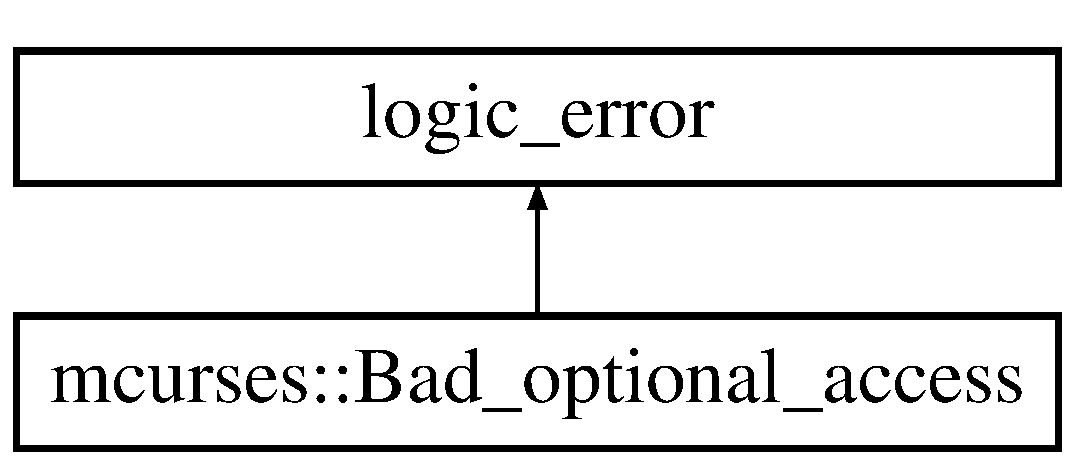
\includegraphics[height=2.000000cm]{classmcurses_1_1Bad__optional__access}
\end{center}
\end{figure}
\subsection*{Public Member Functions}
\begin{DoxyCompactItemize}
\item 
\hypertarget{classmcurses_1_1Bad__optional__access_a5245b58b8e10e7528fd5331b6af38be5}{}\label{classmcurses_1_1Bad__optional__access_a5245b58b8e10e7528fd5331b6af38be5} 
{\bfseries Bad\+\_\+optional\+\_\+access} (const char $\ast$what)
\end{DoxyCompactItemize}


\subsection{Detailed Description}
Exception for use when an empty Optional$<$\+T$>$ object is accessed. 

The documentation for this class was generated from the following file\+:\begin{DoxyCompactItemize}
\item 
/home/anthony/\+Documents/\+C++/\+Projects/\+Optional/include/\hyperlink{bad__optional__access_8hpp}{bad\+\_\+optional\+\_\+access.\+hpp}\end{DoxyCompactItemize}

\hypertarget{classmcurses_1_1None__t}{}\section{mcurses\+:\+:None\+\_\+t Class Reference}
\label{classmcurses_1_1None__t}\index{mcurses\+::\+None\+\_\+t@{mcurses\+::\+None\+\_\+t}}


Represents \textquotesingle{}no value\textquotesingle{}, or null.  




{\ttfamily \#include $<$none.\+hpp$>$}

\subsection*{Public Member Functions}
\begin{DoxyCompactItemize}
\item 
\hypertarget{classmcurses_1_1None__t_a6e1fb4b6ee221d8d65c68a0c185a60b6}{}\label{classmcurses_1_1None__t_a6e1fb4b6ee221d8d65c68a0c185a60b6} 
\hyperlink{classmcurses_1_1None__t_a6e1fb4b6ee221d8d65c68a0c185a60b6}{operator bool} () const
\begin{DoxyCompactList}\small\item\em Safe bool conversion. \end{DoxyCompactList}\end{DoxyCompactItemize}


\subsection{Detailed Description}
Represents \textquotesingle{}no value\textquotesingle{}, or null. 

The documentation for this class was generated from the following file\+:\begin{DoxyCompactItemize}
\item 
/home/anthony/\+Documents/\+C++/\+Projects/\+Optional/include/\hyperlink{none_8hpp}{none.\+hpp}\end{DoxyCompactItemize}

\hypertarget{classmcurses_1_1Optional}{}\section{mcurses\+:\+:Optional$<$ T $>$ Class Template Reference}
\label{classmcurses_1_1Optional}\index{mcurses\+::\+Optional$<$ T $>$@{mcurses\+::\+Optional$<$ T $>$}}


Wraps a type to provide an optional \textquotesingle{}null\textquotesingle{}, or empty state.  




{\ttfamily \#include $<$optional.\+hpp$>$}

\subsection*{Public Types}
\begin{DoxyCompactItemize}
\item 
\hypertarget{classmcurses_1_1Optional_acde60baa6c9d0875b94825e979eda49c}{}\label{classmcurses_1_1Optional_acde60baa6c9d0875b94825e979eda49c} 
using {\bfseries value\+\_\+type} = T
\item 
\hypertarget{classmcurses_1_1Optional_ab9bbf1c6e9076968c95a185a02a264fc}{}\label{classmcurses_1_1Optional_ab9bbf1c6e9076968c95a185a02a264fc} 
using {\bfseries reference\+\_\+type} = T \&
\item 
\hypertarget{classmcurses_1_1Optional_ad890e95fb87a634a20be4c303667dcf8}{}\label{classmcurses_1_1Optional_ad890e95fb87a634a20be4c303667dcf8} 
using {\bfseries reference\+\_\+const\+\_\+type} = const T \&
\item 
\hypertarget{classmcurses_1_1Optional_a58c2635e4aa8b4fe4ae1edd119689587}{}\label{classmcurses_1_1Optional_a58c2635e4aa8b4fe4ae1edd119689587} 
using {\bfseries rval\+\_\+reference\+\_\+type} = T \&\&
\item 
\hypertarget{classmcurses_1_1Optional_a8fd6d3594afac4a3e16017a39022db71}{}\label{classmcurses_1_1Optional_a8fd6d3594afac4a3e16017a39022db71} 
using {\bfseries pointer\+\_\+type} = T $\ast$
\item 
\hypertarget{classmcurses_1_1Optional_a0ea30d61700c90c149f241ec16bb585c}{}\label{classmcurses_1_1Optional_a0ea30d61700c90c149f241ec16bb585c} 
using {\bfseries pointer\+\_\+const\+\_\+type} = const T $\ast$
\end{DoxyCompactItemize}
\subsection*{Public Member Functions}
\begin{DoxyCompactItemize}
\item 
\hyperlink{classmcurses_1_1Optional_a623c4f75b05b17ec7ad6d80faa302a5b}{Optional} () noexcept
\begin{DoxyCompactList}\small\item\em Default constructs an \hyperlink{classmcurses_1_1Optional}{Optional}. \end{DoxyCompactList}\item 
\hyperlink{classmcurses_1_1Optional_a59e637ea31df67b8a2453597603b1493}{Optional} (\hyperlink{classmcurses_1_1None__t}{None\+\_\+t} n) noexcept
\begin{DoxyCompactList}\small\item\em Constructs an uninitialized \hyperlink{classmcurses_1_1Optional}{Optional}. \end{DoxyCompactList}\item 
\hyperlink{classmcurses_1_1Optional_a337b6aa5d069a287cb76867b912dfb47}{Optional} (const T \&\hyperlink{classmcurses_1_1Optional_ad366988d0311c9f6d4de369f222f248f}{value})
\begin{DoxyCompactList}\small\item\em Constructs an initialized \hyperlink{classmcurses_1_1Optional}{Optional} from a T object. \end{DoxyCompactList}\item 
\hyperlink{classmcurses_1_1Optional_acacbd9b1e8a927de478bff6daea6bb96}{Optional} (T \&\&\hyperlink{classmcurses_1_1Optional_ad366988d0311c9f6d4de369f222f248f}{value})
\begin{DoxyCompactList}\small\item\em Constructs an initialized \hyperlink{classmcurses_1_1Optional}{Optional} from a moveable T object. \end{DoxyCompactList}\item 
\hyperlink{classmcurses_1_1Optional_ae0408366bfb3d0b11ba60004871b863e}{Optional} (bool condition, const T \&\hyperlink{classmcurses_1_1Optional_ad366988d0311c9f6d4de369f222f248f}{value})
\begin{DoxyCompactList}\small\item\em Conditionally constructs an initialized \hyperlink{classmcurses_1_1Optional}{Optional}. \end{DoxyCompactList}\item 
\hyperlink{classmcurses_1_1Optional_a53b4829b1acfd54744d6dd8edb6dc2dc}{Optional} (bool condition, T \&\&\hyperlink{classmcurses_1_1Optional_ad366988d0311c9f6d4de369f222f248f}{value})
\begin{DoxyCompactList}\small\item\em Conditionally constructs an \hyperlink{classmcurses_1_1Optional}{Optional} from a moveable T object. \end{DoxyCompactList}\item 
\hyperlink{classmcurses_1_1Optional_a54206fd5a298d201a94fcbf869442169}{Optional} (const \hyperlink{classmcurses_1_1Optional}{Optional} \&rhs)
\begin{DoxyCompactList}\small\item\em Copy constructs an \hyperlink{classmcurses_1_1Optional}{Optional}. \end{DoxyCompactList}\item 
\hyperlink{classmcurses_1_1Optional_a4f9963abeb921ad1b51bbb176fe1e8fd}{Optional} (\hyperlink{classmcurses_1_1Optional}{Optional} \&\&rhs) noexcept
\begin{DoxyCompactList}\small\item\em Move constructs an \hyperlink{classmcurses_1_1Optional}{Optional}. \end{DoxyCompactList}\item 
{\footnotesize template$<$typename U $>$ }\\\hyperlink{classmcurses_1_1Optional_aa89d00c7dcd0b47c2b8fb5ac077795c4}{Optional} (const \hyperlink{classmcurses_1_1Optional}{Optional}$<$ U $>$ \&rhs)
\begin{DoxyCompactList}\small\item\em Copy constructs from implicitly convertible type. \end{DoxyCompactList}\item 
{\footnotesize template$<$typename U $>$ }\\\hyperlink{classmcurses_1_1Optional_a8818f33dbbe44f276c8ba36b83d4b4f6}{Optional} (\hyperlink{classmcurses_1_1Optional}{Optional}$<$ U $>$ \&\&rhs)
\begin{DoxyCompactList}\small\item\em Move constructs from implicitly convertible type. \end{DoxyCompactList}\item 
\hyperlink{classmcurses_1_1Optional}{Optional} \& \hyperlink{classmcurses_1_1Optional_ab76004970466959aaa1ae03255db9bf3}{operator=} (const \hyperlink{classmcurses_1_1Optional}{Optional} \&rhs)
\begin{DoxyCompactList}\small\item\em Copy assignment operator. \end{DoxyCompactList}\item 
\hyperlink{classmcurses_1_1Optional}{Optional} \& \hyperlink{classmcurses_1_1Optional_aae2fb9089d2d969590c3d666339cb1a4}{operator=} (\hyperlink{classmcurses_1_1Optional}{Optional} \&\&rhs) noexcept
\begin{DoxyCompactList}\small\item\em Move assignement operator. \end{DoxyCompactList}\item 
\hyperlink{classmcurses_1_1Optional}{Optional} \& \hyperlink{classmcurses_1_1Optional_a5d3515e3b7ce25aa5f5f5d4c08c1b35e}{operator=} (\hyperlink{classmcurses_1_1None__t}{None\+\_\+t} n) noexcept
\begin{DoxyCompactList}\small\item\em \hyperlink{classmcurses_1_1None__t}{None\+\_\+t} assignement operator. \end{DoxyCompactList}\item 
\hyperlink{classmcurses_1_1Optional}{Optional} \& \hyperlink{classmcurses_1_1Optional_ac77b0ca69b51f7d176983812d95c0807}{operator=} (const T \&\hyperlink{classmcurses_1_1Optional_ad366988d0311c9f6d4de369f222f248f}{value})
\begin{DoxyCompactList}\small\item\em Value copy assignment operator. \end{DoxyCompactList}\item 
\hyperlink{classmcurses_1_1Optional}{Optional} \& \hyperlink{classmcurses_1_1Optional_a023f00ae051bce4f61885e8bbfd14106}{operator=} (T \&\&\hyperlink{classmcurses_1_1Optional_ad366988d0311c9f6d4de369f222f248f}{value})
\begin{DoxyCompactList}\small\item\em Value move assignment operator. \end{DoxyCompactList}\item 
{\footnotesize template$<$typename U $>$ }\\\hyperlink{classmcurses_1_1Optional}{Optional} \& \hyperlink{classmcurses_1_1Optional_a3cb153eb9365b4fc64616d7505465ed8}{operator=} (const \hyperlink{classmcurses_1_1Optional}{Optional}$<$ U $>$ \&rhs)
\begin{DoxyCompactList}\small\item\em Converting copy assignment operator. \end{DoxyCompactList}\item 
{\footnotesize template$<$typename U $>$ }\\\hyperlink{classmcurses_1_1Optional}{Optional} \& \hyperlink{classmcurses_1_1Optional_a08e3433ed663644a0f6f7148197df952}{operator=} (\hyperlink{classmcurses_1_1Optional}{Optional}$<$ U $>$ \&\&rhs)
\begin{DoxyCompactList}\small\item\em Converting move assignment operator. \end{DoxyCompactList}\item 
{\footnotesize template$<$typename... Args$>$ }\\void \hyperlink{classmcurses_1_1Optional_ad61d5e9b20d4824e064f528772e9b805}{emplace} (Args \&\&... args)
\begin{DoxyCompactList}\small\item\em Directly construct a value inside of an existing \hyperlink{classmcurses_1_1Optional}{Optional}. \end{DoxyCompactList}\item 
const T \& \hyperlink{classmcurses_1_1Optional_ac85ab4b82668d46e40f0ad02b83d047e}{get} () const
\begin{DoxyCompactList}\small\item\em Returns a reference to the held value. \end{DoxyCompactList}\item 
T \& \hyperlink{classmcurses_1_1Optional_a353d8df8a75234d372b3a0b0027f2afd}{get} ()
\begin{DoxyCompactList}\small\item\em Returns a reference to the held value. \end{DoxyCompactList}\item 
const T $\ast$ \hyperlink{classmcurses_1_1Optional_a4b2038d37bb6a17cac2904d7c82ce156}{operator-\/$>$} () const
\begin{DoxyCompactList}\small\item\em Member access overload to underlying object. \end{DoxyCompactList}\item 
T $\ast$ \hyperlink{classmcurses_1_1Optional_a64ff247dad4e237f9e16c073174ba6be}{operator-\/$>$} ()
\begin{DoxyCompactList}\small\item\em Member access overload to underlying object. \end{DoxyCompactList}\item 
const T \& \hyperlink{classmcurses_1_1Optional_a080bc167c71a50bdbe27944c2e9b6019}{operator$\ast$} () const \&
\begin{DoxyCompactList}\small\item\em Provides direct access to the underlying object. \end{DoxyCompactList}\item 
T \& \hyperlink{classmcurses_1_1Optional_a2f816c249fc38f69c5c395fdf7d41ca8}{operator$\ast$} () \&
\begin{DoxyCompactList}\small\item\em Provides direct access to the underlying object. \end{DoxyCompactList}\item 
T \&\& \hyperlink{classmcurses_1_1Optional_aba889d24a53535305844ebcae23e6604}{operator$\ast$} () \&\&
\begin{DoxyCompactList}\small\item\em Provides direct access to the underlying object. \end{DoxyCompactList}\item 
const T \& \hyperlink{classmcurses_1_1Optional_ad366988d0311c9f6d4de369f222f248f}{value} () const \&
\begin{DoxyCompactList}\small\item\em Direct access to the underlying object, or throw exception. \end{DoxyCompactList}\item 
T \& \hyperlink{classmcurses_1_1Optional_ab94cd795bbc0dc263d61a2b49cd79084}{value} () \&
\begin{DoxyCompactList}\small\item\em Direct access to the underlying object, or throw exception. \end{DoxyCompactList}\item 
T \&\& \hyperlink{classmcurses_1_1Optional_a0d09d596f54af6693bedcf5dc12e6d3b}{value} () \&\&
\begin{DoxyCompactList}\small\item\em Direct access to the underlying object, or throw exception. \end{DoxyCompactList}\item 
{\footnotesize template$<$typename U $>$ }\\T \hyperlink{classmcurses_1_1Optional_a047c51eb457fd6de52987bf991935f01}{value\+\_\+or} (U \&\&val) const \&
\begin{DoxyCompactList}\small\item\em Direct access to the underlying object, or return {\ttfamily val}. Returns {\ttfamily val} if $\ast$this is uninitialized, otherwise returns a reference to the value stored in $\ast$this. Overloaded on const \&. \end{DoxyCompactList}\item 
{\footnotesize template$<$typename U $>$ }\\T \hyperlink{classmcurses_1_1Optional_aff211e864bc5bda6bc5b72298cdbadd3}{value\+\_\+or} (U \&\&val) \&\&
\begin{DoxyCompactList}\small\item\em Direct access to the underlying object, or return {\ttfamily val}. Returns {\ttfamily val} if $\ast$this is uninitialized, otherwise returns an r-\/value reference to the value stored in $\ast$this. Overloaded on \&\&. \end{DoxyCompactList}\item 
{\footnotesize template$<$typename F $>$ }\\T \hyperlink{classmcurses_1_1Optional_aa5a4cbc8fd315e360e6fcb6dc4e55c07}{value\+\_\+or\+\_\+eval} (F func) const \&
\begin{DoxyCompactList}\small\item\em Direct access to the underlying object, or evaluate {\ttfamily func} and return its value. \end{DoxyCompactList}\item 
{\footnotesize template$<$typename F $>$ }\\T \hyperlink{classmcurses_1_1Optional_ab90365e7ea0a567427f174085931caa4}{value\+\_\+or\+\_\+eval} (F func) \&\&
\begin{DoxyCompactList}\small\item\em Direct access to the underlying object, or evaluate {\ttfamily func} and return its value. \end{DoxyCompactList}\item 
const T $\ast$ \hyperlink{classmcurses_1_1Optional_ac1c01b2ccf9aa96c1e5f91d78bdbc928}{get\+\_\+ptr} () const
\begin{DoxyCompactList}\small\item\em Access to the underlying object\textquotesingle{}s pointer. \end{DoxyCompactList}\item 
T $\ast$ \hyperlink{classmcurses_1_1Optional_a7f9c56ad08329b814a314d741e92fa59}{get\+\_\+ptr} ()
\begin{DoxyCompactList}\small\item\em Access to the underlying object\textquotesingle{}s pointer. \end{DoxyCompactList}\item 
\hyperlink{classmcurses_1_1Optional_ae9ac980d14dea230fdf8e1fbb3501eb4}{operator bool} () const noexcept
\begin{DoxyCompactList}\small\item\em Safe conversion to bool. \end{DoxyCompactList}\item 
bool \hyperlink{classmcurses_1_1Optional_a4d864144db0c48ea381b6582214f256b}{operator!} () const noexcept
\begin{DoxyCompactList}\small\item\em Convinience function. \end{DoxyCompactList}\end{DoxyCompactItemize}
\subsection*{Friends}
\begin{DoxyCompactItemize}
\item 
\hypertarget{classmcurses_1_1Optional_a1765268b663a7e1bce2246dec366ac57}{}\label{classmcurses_1_1Optional_a1765268b663a7e1bce2246dec366ac57} 
{\footnotesize template$<$typename U $>$ }\\class {\bfseries Optional}
\end{DoxyCompactItemize}


\subsection{Detailed Description}
\subsubsection*{template$<$typename T$>$\newline
class mcurses\+::\+Optional$<$ T $>$}

Wraps a type to provide an optional \textquotesingle{}null\textquotesingle{}, or empty state. 

A wrapped object is accessed by dereferencing an \hyperlink{classmcurses_1_1Optional}{Optional} object. \hyperlink{classmcurses_1_1Optional}{Optional} objects can be tested as a boolean for whether or not they contain a value. Useful when 0, -\/1, or default constructed does not suffice for \textquotesingle{}no value\textquotesingle{}.

Typical usage\+: 
\begin{DoxyCode}
Optional<int> opt\_i\{5\};
\textcolor{keywordflow}{if}(opt\_i) \{
    foo(*opt\_i);
\}
\end{DoxyCode}
 

\subsection{Constructor \& Destructor Documentation}
\hypertarget{classmcurses_1_1Optional_a623c4f75b05b17ec7ad6d80faa302a5b}{}\label{classmcurses_1_1Optional_a623c4f75b05b17ec7ad6d80faa302a5b} 
\index{mcurses\+::\+Optional@{mcurses\+::\+Optional}!Optional@{Optional}}
\index{Optional@{Optional}!mcurses\+::\+Optional@{mcurses\+::\+Optional}}
\subsubsection{\texorpdfstring{Optional()}{Optional()}\hspace{0.1cm}{\footnotesize\ttfamily [1/10]}}
{\footnotesize\ttfamily template$<$typename T$>$ \\
\hyperlink{classmcurses_1_1Optional}{mcurses\+::\+Optional}$<$ T $>$\+::\hyperlink{classmcurses_1_1Optional}{Optional} (\begin{DoxyParamCaption}{ }\end{DoxyParamCaption})\hspace{0.3cm}{\ttfamily [inline]}, {\ttfamily [noexcept]}}



Default constructs an \hyperlink{classmcurses_1_1Optional}{Optional}. 

$\ast$this is {\itshape not} initialized, T\textquotesingle{}s default constructor is {\itshape not} called. \hypertarget{classmcurses_1_1Optional_a59e637ea31df67b8a2453597603b1493}{}\label{classmcurses_1_1Optional_a59e637ea31df67b8a2453597603b1493} 
\index{mcurses\+::\+Optional@{mcurses\+::\+Optional}!Optional@{Optional}}
\index{Optional@{Optional}!mcurses\+::\+Optional@{mcurses\+::\+Optional}}
\subsubsection{\texorpdfstring{Optional()}{Optional()}\hspace{0.1cm}{\footnotesize\ttfamily [2/10]}}
{\footnotesize\ttfamily template$<$typename T$>$ \\
\hyperlink{classmcurses_1_1Optional}{mcurses\+::\+Optional}$<$ T $>$\+::\hyperlink{classmcurses_1_1Optional}{Optional} (\begin{DoxyParamCaption}\item[{\hyperlink{classmcurses_1_1None__t}{None\+\_\+t}}]{n }\end{DoxyParamCaption})\hspace{0.3cm}{\ttfamily [inline]}, {\ttfamily [noexcept]}}



Constructs an uninitialized \hyperlink{classmcurses_1_1Optional}{Optional}. 

$\ast$this is {\itshape not} initialized, T\textquotesingle{}s default constrcutor is {\itshape not} called. 
\begin{DoxyParams}{Parameters}
{\em n} & Use \hyperlink{namespacemcurses_a3fd18c73e6d453dcdfdd1fcdaf9bb0d7}{mcurses\+::none} provided in \hyperlink{none_8hpp}{none.\+hpp}. \\
\hline
\end{DoxyParams}
\begin{DoxySeeAlso}{See also}
\hyperlink{namespacemcurses_a3fd18c73e6d453dcdfdd1fcdaf9bb0d7}{none} 
\end{DoxySeeAlso}
\hypertarget{classmcurses_1_1Optional_a337b6aa5d069a287cb76867b912dfb47}{}\label{classmcurses_1_1Optional_a337b6aa5d069a287cb76867b912dfb47} 
\index{mcurses\+::\+Optional@{mcurses\+::\+Optional}!Optional@{Optional}}
\index{Optional@{Optional}!mcurses\+::\+Optional@{mcurses\+::\+Optional}}
\subsubsection{\texorpdfstring{Optional()}{Optional()}\hspace{0.1cm}{\footnotesize\ttfamily [3/10]}}
{\footnotesize\ttfamily template$<$typename T$>$ \\
\hyperlink{classmcurses_1_1Optional}{mcurses\+::\+Optional}$<$ T $>$\+::\hyperlink{classmcurses_1_1Optional}{Optional} (\begin{DoxyParamCaption}\item[{const T \&}]{value }\end{DoxyParamCaption})\hspace{0.3cm}{\ttfamily [inline]}}



Constructs an initialized \hyperlink{classmcurses_1_1Optional}{Optional} from a T object. 

$\ast$this is initialized with a copy of {\ttfamily value}. 
\begin{DoxyParams}{Parameters}
{\em value} & Value which is copied into the \hyperlink{classmcurses_1_1Optional}{Optional}. \\
\hline
\end{DoxyParams}
\hypertarget{classmcurses_1_1Optional_acacbd9b1e8a927de478bff6daea6bb96}{}\label{classmcurses_1_1Optional_acacbd9b1e8a927de478bff6daea6bb96} 
\index{mcurses\+::\+Optional@{mcurses\+::\+Optional}!Optional@{Optional}}
\index{Optional@{Optional}!mcurses\+::\+Optional@{mcurses\+::\+Optional}}
\subsubsection{\texorpdfstring{Optional()}{Optional()}\hspace{0.1cm}{\footnotesize\ttfamily [4/10]}}
{\footnotesize\ttfamily template$<$typename T$>$ \\
\hyperlink{classmcurses_1_1Optional}{mcurses\+::\+Optional}$<$ T $>$\+::\hyperlink{classmcurses_1_1Optional}{Optional} (\begin{DoxyParamCaption}\item[{T \&\&}]{value }\end{DoxyParamCaption})\hspace{0.3cm}{\ttfamily [inline]}}



Constructs an initialized \hyperlink{classmcurses_1_1Optional}{Optional} from a moveable T object. 

{\ttfamily value} is move constructed into the \hyperlink{classmcurses_1_1Optional}{Optional} object. 
\begin{DoxyParams}{Parameters}
{\em value} & Value which is moved into the \hyperlink{classmcurses_1_1Optional}{Optional}. \\
\hline
\end{DoxyParams}
\hypertarget{classmcurses_1_1Optional_ae0408366bfb3d0b11ba60004871b863e}{}\label{classmcurses_1_1Optional_ae0408366bfb3d0b11ba60004871b863e} 
\index{mcurses\+::\+Optional@{mcurses\+::\+Optional}!Optional@{Optional}}
\index{Optional@{Optional}!mcurses\+::\+Optional@{mcurses\+::\+Optional}}
\subsubsection{\texorpdfstring{Optional()}{Optional()}\hspace{0.1cm}{\footnotesize\ttfamily [5/10]}}
{\footnotesize\ttfamily template$<$typename T$>$ \\
\hyperlink{classmcurses_1_1Optional}{mcurses\+::\+Optional}$<$ T $>$\+::\hyperlink{classmcurses_1_1Optional}{Optional} (\begin{DoxyParamCaption}\item[{bool}]{condition,  }\item[{const T \&}]{value }\end{DoxyParamCaption})\hspace{0.3cm}{\ttfamily [inline]}}



Conditionally constructs an initialized \hyperlink{classmcurses_1_1Optional}{Optional}. 

If condition is true, {\ttfamily value} is copy constructed into $\ast$this, otherwise $\ast$this is not initialized. 
\begin{DoxyParams}{Parameters}
{\em condition} & Determines if \hyperlink{classmcurses_1_1Optional}{Optional} is initialized or not. \\
\hline
{\em value} & Object copied into $\ast$this if {\ttfamily condition} is true. \\
\hline
\end{DoxyParams}
\hypertarget{classmcurses_1_1Optional_a53b4829b1acfd54744d6dd8edb6dc2dc}{}\label{classmcurses_1_1Optional_a53b4829b1acfd54744d6dd8edb6dc2dc} 
\index{mcurses\+::\+Optional@{mcurses\+::\+Optional}!Optional@{Optional}}
\index{Optional@{Optional}!mcurses\+::\+Optional@{mcurses\+::\+Optional}}
\subsubsection{\texorpdfstring{Optional()}{Optional()}\hspace{0.1cm}{\footnotesize\ttfamily [6/10]}}
{\footnotesize\ttfamily template$<$typename T$>$ \\
\hyperlink{classmcurses_1_1Optional}{mcurses\+::\+Optional}$<$ T $>$\+::\hyperlink{classmcurses_1_1Optional}{Optional} (\begin{DoxyParamCaption}\item[{bool}]{condition,  }\item[{T \&\&}]{value }\end{DoxyParamCaption})\hspace{0.3cm}{\ttfamily [inline]}}



Conditionally constructs an \hyperlink{classmcurses_1_1Optional}{Optional} from a moveable T object. 

If condition is true, {\ttfamily value} is move constructed into $\ast$this, otherwise $\ast$this is not initialized. 
\begin{DoxyParams}{Parameters}
{\em condition} & Determines if \hyperlink{classmcurses_1_1Optional}{Optional} is initialized or not. \\
\hline
{\em value} & Object moved into $\ast$this if {\ttfamily condition} is true. \\
\hline
\end{DoxyParams}
\hypertarget{classmcurses_1_1Optional_a54206fd5a298d201a94fcbf869442169}{}\label{classmcurses_1_1Optional_a54206fd5a298d201a94fcbf869442169} 
\index{mcurses\+::\+Optional@{mcurses\+::\+Optional}!Optional@{Optional}}
\index{Optional@{Optional}!mcurses\+::\+Optional@{mcurses\+::\+Optional}}
\subsubsection{\texorpdfstring{Optional()}{Optional()}\hspace{0.1cm}{\footnotesize\ttfamily [7/10]}}
{\footnotesize\ttfamily template$<$typename T$>$ \\
\hyperlink{classmcurses_1_1Optional}{mcurses\+::\+Optional}$<$ T $>$\+::\hyperlink{classmcurses_1_1Optional}{Optional} (\begin{DoxyParamCaption}\item[{const \hyperlink{classmcurses_1_1Optional}{Optional}$<$ T $>$ \&}]{rhs }\end{DoxyParamCaption})\hspace{0.3cm}{\ttfamily [inline]}}



Copy constructs an \hyperlink{classmcurses_1_1Optional}{Optional}. 

If {\ttfamily rhs} is initialized, then a copy of its value will be constructed within $\ast$this, and $\ast$this will be initialized, otherwise $\ast$this is default constructed. 
\begin{DoxyParams}{Parameters}
{\em rhs} & \hyperlink{classmcurses_1_1Optional}{Optional} to copy, T must be copy constructible. \\
\hline
\end{DoxyParams}
\hypertarget{classmcurses_1_1Optional_a4f9963abeb921ad1b51bbb176fe1e8fd}{}\label{classmcurses_1_1Optional_a4f9963abeb921ad1b51bbb176fe1e8fd} 
\index{mcurses\+::\+Optional@{mcurses\+::\+Optional}!Optional@{Optional}}
\index{Optional@{Optional}!mcurses\+::\+Optional@{mcurses\+::\+Optional}}
\subsubsection{\texorpdfstring{Optional()}{Optional()}\hspace{0.1cm}{\footnotesize\ttfamily [8/10]}}
{\footnotesize\ttfamily template$<$typename T$>$ \\
\hyperlink{classmcurses_1_1Optional}{mcurses\+::\+Optional}$<$ T $>$\+::\hyperlink{classmcurses_1_1Optional}{Optional} (\begin{DoxyParamCaption}\item[{\hyperlink{classmcurses_1_1Optional}{Optional}$<$ T $>$ \&\&}]{rhs }\end{DoxyParamCaption})\hspace{0.3cm}{\ttfamily [inline]}, {\ttfamily [noexcept]}}



Move constructs an \hyperlink{classmcurses_1_1Optional}{Optional}. 

If {\ttfamily rhs} is initialized, then its internally held value is moved into $\ast$this, and {\ttfamily rhs} will be empty, otherwise $\ast$this is default constructed. 
\begin{DoxyParams}{Parameters}
{\em rhs} & \hyperlink{classmcurses_1_1Optional}{Optional} to move, T must be move constructible. \\
\hline
\end{DoxyParams}
\hypertarget{classmcurses_1_1Optional_aa89d00c7dcd0b47c2b8fb5ac077795c4}{}\label{classmcurses_1_1Optional_aa89d00c7dcd0b47c2b8fb5ac077795c4} 
\index{mcurses\+::\+Optional@{mcurses\+::\+Optional}!Optional@{Optional}}
\index{Optional@{Optional}!mcurses\+::\+Optional@{mcurses\+::\+Optional}}
\subsubsection{\texorpdfstring{Optional()}{Optional()}\hspace{0.1cm}{\footnotesize\ttfamily [9/10]}}
{\footnotesize\ttfamily template$<$typename T$>$ \\
template$<$typename U $>$ \\
\hyperlink{classmcurses_1_1Optional}{mcurses\+::\+Optional}$<$ T $>$\+::\hyperlink{classmcurses_1_1Optional}{Optional} (\begin{DoxyParamCaption}\item[{const \hyperlink{classmcurses_1_1Optional}{Optional}$<$ U $>$ \&}]{rhs }\end{DoxyParamCaption})\hspace{0.3cm}{\ttfamily [inline]}, {\ttfamily [explicit]}}



Copy constructs from implicitly convertible type. 

If {\ttfamily rhs} is initialized and U is implicitly convertible to T, then $\ast$this is initialized with a copy of {\ttfamily rhs}. 
\begin{DoxyParams}{Parameters}
{\em rhs} & Object to be copied into $\ast$this. \\
\hline
\end{DoxyParams}
\hypertarget{classmcurses_1_1Optional_a8818f33dbbe44f276c8ba36b83d4b4f6}{}\label{classmcurses_1_1Optional_a8818f33dbbe44f276c8ba36b83d4b4f6} 
\index{mcurses\+::\+Optional@{mcurses\+::\+Optional}!Optional@{Optional}}
\index{Optional@{Optional}!mcurses\+::\+Optional@{mcurses\+::\+Optional}}
\subsubsection{\texorpdfstring{Optional()}{Optional()}\hspace{0.1cm}{\footnotesize\ttfamily [10/10]}}
{\footnotesize\ttfamily template$<$typename T$>$ \\
template$<$typename U $>$ \\
\hyperlink{classmcurses_1_1Optional}{mcurses\+::\+Optional}$<$ T $>$\+::\hyperlink{classmcurses_1_1Optional}{Optional} (\begin{DoxyParamCaption}\item[{\hyperlink{classmcurses_1_1Optional}{Optional}$<$ U $>$ \&\&}]{rhs }\end{DoxyParamCaption})\hspace{0.3cm}{\ttfamily [inline]}, {\ttfamily [explicit]}}



Move constructs from implicitly convertible type. 

If {\ttfamily rhs} is initialized and U is implicitly convertible to T, then $\ast$this is initialized with {\ttfamily rhs}. T must have a move constructor defined from type U. 
\begin{DoxyParams}{Parameters}
{\em rhs} & Object to be moved into $\ast$this. \\
\hline
\end{DoxyParams}


\subsection{Member Function Documentation}
\hypertarget{classmcurses_1_1Optional_ad61d5e9b20d4824e064f528772e9b805}{}\label{classmcurses_1_1Optional_ad61d5e9b20d4824e064f528772e9b805} 
\index{mcurses\+::\+Optional@{mcurses\+::\+Optional}!emplace@{emplace}}
\index{emplace@{emplace}!mcurses\+::\+Optional@{mcurses\+::\+Optional}}
\subsubsection{\texorpdfstring{emplace()}{emplace()}}
{\footnotesize\ttfamily template$<$typename T$>$ \\
template$<$typename... Args$>$ \\
void \hyperlink{classmcurses_1_1Optional}{mcurses\+::\+Optional}$<$ T $>$\+::emplace (\begin{DoxyParamCaption}\item[{Args \&\&...}]{args }\end{DoxyParamCaption})\hspace{0.3cm}{\ttfamily [inline]}}



Directly construct a value inside of an existing \hyperlink{classmcurses_1_1Optional}{Optional}. 

If $\ast$this is initialized, the held object is destroyed. The {\ttfamily args} are forwarded to the constructor of T. \hypertarget{classmcurses_1_1Optional_ac85ab4b82668d46e40f0ad02b83d047e}{}\label{classmcurses_1_1Optional_ac85ab4b82668d46e40f0ad02b83d047e} 
\index{mcurses\+::\+Optional@{mcurses\+::\+Optional}!get@{get}}
\index{get@{get}!mcurses\+::\+Optional@{mcurses\+::\+Optional}}
\subsubsection{\texorpdfstring{get()}{get()}\hspace{0.1cm}{\footnotesize\ttfamily [1/2]}}
{\footnotesize\ttfamily template$<$typename T$>$ \\
const T\& \hyperlink{classmcurses_1_1Optional}{mcurses\+::\+Optional}$<$ T $>$\+::get (\begin{DoxyParamCaption}{ }\end{DoxyParamCaption}) const\hspace{0.3cm}{\ttfamily [inline]}}



Returns a reference to the held value. 

Undefined if $\ast$this is uninitialized. \begin{DoxyReturn}{Returns}
const reference to the underlying object. 
\end{DoxyReturn}
\hypertarget{classmcurses_1_1Optional_a353d8df8a75234d372b3a0b0027f2afd}{}\label{classmcurses_1_1Optional_a353d8df8a75234d372b3a0b0027f2afd} 
\index{mcurses\+::\+Optional@{mcurses\+::\+Optional}!get@{get}}
\index{get@{get}!mcurses\+::\+Optional@{mcurses\+::\+Optional}}
\subsubsection{\texorpdfstring{get()}{get()}\hspace{0.1cm}{\footnotesize\ttfamily [2/2]}}
{\footnotesize\ttfamily template$<$typename T$>$ \\
T\& \hyperlink{classmcurses_1_1Optional}{mcurses\+::\+Optional}$<$ T $>$\+::get (\begin{DoxyParamCaption}{ }\end{DoxyParamCaption})\hspace{0.3cm}{\ttfamily [inline]}}



Returns a reference to the held value. 

Undefined if $\ast$this is uninitialized. \begin{DoxyReturn}{Returns}
Reference to the underlying object. 
\end{DoxyReturn}
\hypertarget{classmcurses_1_1Optional_ac1c01b2ccf9aa96c1e5f91d78bdbc928}{}\label{classmcurses_1_1Optional_ac1c01b2ccf9aa96c1e5f91d78bdbc928} 
\index{mcurses\+::\+Optional@{mcurses\+::\+Optional}!get\+\_\+ptr@{get\+\_\+ptr}}
\index{get\+\_\+ptr@{get\+\_\+ptr}!mcurses\+::\+Optional@{mcurses\+::\+Optional}}
\subsubsection{\texorpdfstring{get\+\_\+ptr()}{get\_ptr()}\hspace{0.1cm}{\footnotesize\ttfamily [1/2]}}
{\footnotesize\ttfamily template$<$typename T$>$ \\
const T$\ast$ \hyperlink{classmcurses_1_1Optional}{mcurses\+::\+Optional}$<$ T $>$\+::get\+\_\+ptr (\begin{DoxyParamCaption}{ }\end{DoxyParamCaption}) const\hspace{0.3cm}{\ttfamily [inline]}}



Access to the underlying object\textquotesingle{}s pointer. 

$\ast$this still owns the object, do not delete the object via this pointer. \begin{DoxyReturn}{Returns}
const pointer to the underlying object. 
\end{DoxyReturn}
\hypertarget{classmcurses_1_1Optional_a7f9c56ad08329b814a314d741e92fa59}{}\label{classmcurses_1_1Optional_a7f9c56ad08329b814a314d741e92fa59} 
\index{mcurses\+::\+Optional@{mcurses\+::\+Optional}!get\+\_\+ptr@{get\+\_\+ptr}}
\index{get\+\_\+ptr@{get\+\_\+ptr}!mcurses\+::\+Optional@{mcurses\+::\+Optional}}
\subsubsection{\texorpdfstring{get\+\_\+ptr()}{get\_ptr()}\hspace{0.1cm}{\footnotesize\ttfamily [2/2]}}
{\footnotesize\ttfamily template$<$typename T$>$ \\
T$\ast$ \hyperlink{classmcurses_1_1Optional}{mcurses\+::\+Optional}$<$ T $>$\+::get\+\_\+ptr (\begin{DoxyParamCaption}{ }\end{DoxyParamCaption})\hspace{0.3cm}{\ttfamily [inline]}}



Access to the underlying object\textquotesingle{}s pointer. 

$\ast$this still owns the object, do not delete the object via this pointer. \begin{DoxyReturn}{Returns}
Pointer to the underlying object. 
\end{DoxyReturn}
\hypertarget{classmcurses_1_1Optional_ae9ac980d14dea230fdf8e1fbb3501eb4}{}\label{classmcurses_1_1Optional_ae9ac980d14dea230fdf8e1fbb3501eb4} 
\index{mcurses\+::\+Optional@{mcurses\+::\+Optional}!operator bool@{operator bool}}
\index{operator bool@{operator bool}!mcurses\+::\+Optional@{mcurses\+::\+Optional}}
\subsubsection{\texorpdfstring{operator bool()}{operator bool()}}
{\footnotesize\ttfamily template$<$typename T$>$ \\
\hyperlink{classmcurses_1_1Optional}{mcurses\+::\+Optional}$<$ T $>$\+::operator bool (\begin{DoxyParamCaption}{ }\end{DoxyParamCaption}) const\hspace{0.3cm}{\ttfamily [inline]}, {\ttfamily [explicit]}, {\ttfamily [noexcept]}}



Safe conversion to bool. 

\begin{DoxyReturn}{Returns}
True if object contains a value, false otherwise. 
\end{DoxyReturn}
\hypertarget{classmcurses_1_1Optional_a4d864144db0c48ea381b6582214f256b}{}\label{classmcurses_1_1Optional_a4d864144db0c48ea381b6582214f256b} 
\index{mcurses\+::\+Optional@{mcurses\+::\+Optional}!operator"!@{operator"!}}
\index{operator"!@{operator"!}!mcurses\+::\+Optional@{mcurses\+::\+Optional}}
\subsubsection{\texorpdfstring{operator"!()}{operator!()}}
{\footnotesize\ttfamily template$<$typename T$>$ \\
bool \hyperlink{classmcurses_1_1Optional}{mcurses\+::\+Optional}$<$ T $>$\+::operator! (\begin{DoxyParamCaption}{ }\end{DoxyParamCaption}) const\hspace{0.3cm}{\ttfamily [inline]}, {\ttfamily [noexcept]}}



Convinience function. 

Explicit operator bool makes ! operation verbose with !bool(opt). \begin{DoxyReturn}{Returns}
Opposite of operator bool. 
\end{DoxyReturn}
\hypertarget{classmcurses_1_1Optional_a080bc167c71a50bdbe27944c2e9b6019}{}\label{classmcurses_1_1Optional_a080bc167c71a50bdbe27944c2e9b6019} 
\index{mcurses\+::\+Optional@{mcurses\+::\+Optional}!operator$\ast$@{operator$\ast$}}
\index{operator$\ast$@{operator$\ast$}!mcurses\+::\+Optional@{mcurses\+::\+Optional}}
\subsubsection{\texorpdfstring{operator$\ast$()}{operator*()}\hspace{0.1cm}{\footnotesize\ttfamily [1/3]}}
{\footnotesize\ttfamily template$<$typename T$>$ \\
const T\& \hyperlink{classmcurses_1_1Optional}{mcurses\+::\+Optional}$<$ T $>$\+::operator$\ast$ (\begin{DoxyParamCaption}{ }\end{DoxyParamCaption}) const\hspace{0.3cm}{\ttfamily [inline]}}



Provides direct access to the underlying object. 

Undefined if $\ast$this is uninitialized. Overloaded on const \&. \begin{DoxyReturn}{Returns}
const l-\/value reference to the held object. 
\end{DoxyReturn}
\hypertarget{classmcurses_1_1Optional_a2f816c249fc38f69c5c395fdf7d41ca8}{}\label{classmcurses_1_1Optional_a2f816c249fc38f69c5c395fdf7d41ca8} 
\index{mcurses\+::\+Optional@{mcurses\+::\+Optional}!operator$\ast$@{operator$\ast$}}
\index{operator$\ast$@{operator$\ast$}!mcurses\+::\+Optional@{mcurses\+::\+Optional}}
\subsubsection{\texorpdfstring{operator$\ast$()}{operator*()}\hspace{0.1cm}{\footnotesize\ttfamily [2/3]}}
{\footnotesize\ttfamily template$<$typename T$>$ \\
T\& \hyperlink{classmcurses_1_1Optional}{mcurses\+::\+Optional}$<$ T $>$\+::operator$\ast$ (\begin{DoxyParamCaption}{ }\end{DoxyParamCaption})\hspace{0.3cm}{\ttfamily [inline]}}



Provides direct access to the underlying object. 

Undefined if $\ast$this is uninitialized. Overloaded on \&. \begin{DoxyReturn}{Returns}
l-\/value reference to the held object. 
\end{DoxyReturn}
\hypertarget{classmcurses_1_1Optional_aba889d24a53535305844ebcae23e6604}{}\label{classmcurses_1_1Optional_aba889d24a53535305844ebcae23e6604} 
\index{mcurses\+::\+Optional@{mcurses\+::\+Optional}!operator$\ast$@{operator$\ast$}}
\index{operator$\ast$@{operator$\ast$}!mcurses\+::\+Optional@{mcurses\+::\+Optional}}
\subsubsection{\texorpdfstring{operator$\ast$()}{operator*()}\hspace{0.1cm}{\footnotesize\ttfamily [3/3]}}
{\footnotesize\ttfamily template$<$typename T$>$ \\
T\&\& \hyperlink{classmcurses_1_1Optional}{mcurses\+::\+Optional}$<$ T $>$\+::operator$\ast$ (\begin{DoxyParamCaption}{ }\end{DoxyParamCaption})\hspace{0.3cm}{\ttfamily [inline]}}



Provides direct access to the underlying object. 

Undefined if $\ast$this is uninitialized. Overloaded on \&\&. \begin{DoxyReturn}{Returns}
r-\/value reference to the underlying object 
\end{DoxyReturn}
\hypertarget{classmcurses_1_1Optional_a4b2038d37bb6a17cac2904d7c82ce156}{}\label{classmcurses_1_1Optional_a4b2038d37bb6a17cac2904d7c82ce156} 
\index{mcurses\+::\+Optional@{mcurses\+::\+Optional}!operator-\/$>$@{operator-\/$>$}}
\index{operator-\/$>$@{operator-\/$>$}!mcurses\+::\+Optional@{mcurses\+::\+Optional}}
\subsubsection{\texorpdfstring{operator-\/$>$()}{operator->()}\hspace{0.1cm}{\footnotesize\ttfamily [1/2]}}
{\footnotesize\ttfamily template$<$typename T$>$ \\
const T$\ast$ \hyperlink{classmcurses_1_1Optional}{mcurses\+::\+Optional}$<$ T $>$\+::operator-\/$>$ (\begin{DoxyParamCaption}{ }\end{DoxyParamCaption}) const\hspace{0.3cm}{\ttfamily [inline]}}



Member access overload to underlying object. 

Undefined if $\ast$this is uninitialized. \begin{DoxyReturn}{Returns}
const pointer to the underlying object. 
\end{DoxyReturn}
\hypertarget{classmcurses_1_1Optional_a64ff247dad4e237f9e16c073174ba6be}{}\label{classmcurses_1_1Optional_a64ff247dad4e237f9e16c073174ba6be} 
\index{mcurses\+::\+Optional@{mcurses\+::\+Optional}!operator-\/$>$@{operator-\/$>$}}
\index{operator-\/$>$@{operator-\/$>$}!mcurses\+::\+Optional@{mcurses\+::\+Optional}}
\subsubsection{\texorpdfstring{operator-\/$>$()}{operator->()}\hspace{0.1cm}{\footnotesize\ttfamily [2/2]}}
{\footnotesize\ttfamily template$<$typename T$>$ \\
T$\ast$ \hyperlink{classmcurses_1_1Optional}{mcurses\+::\+Optional}$<$ T $>$\+::operator-\/$>$ (\begin{DoxyParamCaption}{ }\end{DoxyParamCaption})\hspace{0.3cm}{\ttfamily [inline]}}



Member access overload to underlying object. 

Undefined if $\ast$this is uninitialized. \begin{DoxyReturn}{Returns}
Pointer to the underlying object. 
\end{DoxyReturn}
\hypertarget{classmcurses_1_1Optional_ab76004970466959aaa1ae03255db9bf3}{}\label{classmcurses_1_1Optional_ab76004970466959aaa1ae03255db9bf3} 
\index{mcurses\+::\+Optional@{mcurses\+::\+Optional}!operator=@{operator=}}
\index{operator=@{operator=}!mcurses\+::\+Optional@{mcurses\+::\+Optional}}
\subsubsection{\texorpdfstring{operator=()}{operator=()}\hspace{0.1cm}{\footnotesize\ttfamily [1/7]}}
{\footnotesize\ttfamily template$<$typename T$>$ \\
\hyperlink{classmcurses_1_1Optional}{Optional}\& \hyperlink{classmcurses_1_1Optional}{mcurses\+::\+Optional}$<$ T $>$\+::operator= (\begin{DoxyParamCaption}\item[{const \hyperlink{classmcurses_1_1Optional}{Optional}$<$ T $>$ \&}]{rhs }\end{DoxyParamCaption})\hspace{0.3cm}{\ttfamily [inline]}}



Copy assignment operator. 

The object held by $\ast$this is destroyed and replaced with the contents of {\ttfamily rhs}. If {\ttfamily rhs} is empty, $\ast$this is left empty. 
\begin{DoxyParams}{Parameters}
{\em rhs} & Object to be copied into $\ast$this. \\
\hline
\end{DoxyParams}
\hypertarget{classmcurses_1_1Optional_aae2fb9089d2d969590c3d666339cb1a4}{}\label{classmcurses_1_1Optional_aae2fb9089d2d969590c3d666339cb1a4} 
\index{mcurses\+::\+Optional@{mcurses\+::\+Optional}!operator=@{operator=}}
\index{operator=@{operator=}!mcurses\+::\+Optional@{mcurses\+::\+Optional}}
\subsubsection{\texorpdfstring{operator=()}{operator=()}\hspace{0.1cm}{\footnotesize\ttfamily [2/7]}}
{\footnotesize\ttfamily template$<$typename T$>$ \\
\hyperlink{classmcurses_1_1Optional}{Optional}\& \hyperlink{classmcurses_1_1Optional}{mcurses\+::\+Optional}$<$ T $>$\+::operator= (\begin{DoxyParamCaption}\item[{\hyperlink{classmcurses_1_1Optional}{Optional}$<$ T $>$ \&\&}]{rhs }\end{DoxyParamCaption})\hspace{0.3cm}{\ttfamily [inline]}, {\ttfamily [noexcept]}}



Move assignement operator. 

The object held by $\ast$this is destroyed and replaced with the contents of {\ttfamily rhs}. If {\ttfamily rhs} is empty, $\ast$this is left empty. rhs is left in an invalid state. 
\begin{DoxyParams}{Parameters}
{\em rhs} & Object to be moved into $\ast$this. \\
\hline
\end{DoxyParams}
\hypertarget{classmcurses_1_1Optional_a5d3515e3b7ce25aa5f5f5d4c08c1b35e}{}\label{classmcurses_1_1Optional_a5d3515e3b7ce25aa5f5f5d4c08c1b35e} 
\index{mcurses\+::\+Optional@{mcurses\+::\+Optional}!operator=@{operator=}}
\index{operator=@{operator=}!mcurses\+::\+Optional@{mcurses\+::\+Optional}}
\subsubsection{\texorpdfstring{operator=()}{operator=()}\hspace{0.1cm}{\footnotesize\ttfamily [3/7]}}
{\footnotesize\ttfamily template$<$typename T$>$ \\
\hyperlink{classmcurses_1_1Optional}{Optional}\& \hyperlink{classmcurses_1_1Optional}{mcurses\+::\+Optional}$<$ T $>$\+::operator= (\begin{DoxyParamCaption}\item[{\hyperlink{classmcurses_1_1None__t}{None\+\_\+t}}]{n }\end{DoxyParamCaption})\hspace{0.3cm}{\ttfamily [inline]}, {\ttfamily [noexcept]}}



\hyperlink{classmcurses_1_1None__t}{None\+\_\+t} assignement operator. 

Leaves $\ast$this in an uninitialized state. If $\ast$this was previously initialized, the held object is destroyed. 
\begin{DoxyParams}{Parameters}
{\em n} & Use \hyperlink{namespacemcurses_a3fd18c73e6d453dcdfdd1fcdaf9bb0d7}{mcurses\+::none} provided in \hyperlink{none_8hpp}{none.\+hpp}. \\
\hline
\end{DoxyParams}
\begin{DoxySeeAlso}{See also}
\hyperlink{namespacemcurses_a3fd18c73e6d453dcdfdd1fcdaf9bb0d7}{none} 
\end{DoxySeeAlso}
\hypertarget{classmcurses_1_1Optional_ac77b0ca69b51f7d176983812d95c0807}{}\label{classmcurses_1_1Optional_ac77b0ca69b51f7d176983812d95c0807} 
\index{mcurses\+::\+Optional@{mcurses\+::\+Optional}!operator=@{operator=}}
\index{operator=@{operator=}!mcurses\+::\+Optional@{mcurses\+::\+Optional}}
\subsubsection{\texorpdfstring{operator=()}{operator=()}\hspace{0.1cm}{\footnotesize\ttfamily [4/7]}}
{\footnotesize\ttfamily template$<$typename T$>$ \\
\hyperlink{classmcurses_1_1Optional}{Optional}\& \hyperlink{classmcurses_1_1Optional}{mcurses\+::\+Optional}$<$ T $>$\+::operator= (\begin{DoxyParamCaption}\item[{const T \&}]{value }\end{DoxyParamCaption})\hspace{0.3cm}{\ttfamily [inline]}}



Value copy assignment operator. 

If $\ast$this is initialized, the object held is destroyed and replaced with a copy of {\ttfamily value}. T must be copy constructible. 
\begin{DoxyParams}{Parameters}
{\em value} & Value to be copied into $\ast$this. \\
\hline
\end{DoxyParams}
\hypertarget{classmcurses_1_1Optional_a023f00ae051bce4f61885e8bbfd14106}{}\label{classmcurses_1_1Optional_a023f00ae051bce4f61885e8bbfd14106} 
\index{mcurses\+::\+Optional@{mcurses\+::\+Optional}!operator=@{operator=}}
\index{operator=@{operator=}!mcurses\+::\+Optional@{mcurses\+::\+Optional}}
\subsubsection{\texorpdfstring{operator=()}{operator=()}\hspace{0.1cm}{\footnotesize\ttfamily [5/7]}}
{\footnotesize\ttfamily template$<$typename T$>$ \\
\hyperlink{classmcurses_1_1Optional}{Optional}\& \hyperlink{classmcurses_1_1Optional}{mcurses\+::\+Optional}$<$ T $>$\+::operator= (\begin{DoxyParamCaption}\item[{T \&\&}]{value }\end{DoxyParamCaption})\hspace{0.3cm}{\ttfamily [inline]}}



Value move assignment operator. 

If $\ast$this is initialized, the object held is destroyed and replaced with {\ttfamily value}. T must be move constructible. 
\begin{DoxyParams}{Parameters}
{\em value} & Value to be moved into $\ast$this. \\
\hline
\end{DoxyParams}
\hypertarget{classmcurses_1_1Optional_a3cb153eb9365b4fc64616d7505465ed8}{}\label{classmcurses_1_1Optional_a3cb153eb9365b4fc64616d7505465ed8} 
\index{mcurses\+::\+Optional@{mcurses\+::\+Optional}!operator=@{operator=}}
\index{operator=@{operator=}!mcurses\+::\+Optional@{mcurses\+::\+Optional}}
\subsubsection{\texorpdfstring{operator=()}{operator=()}\hspace{0.1cm}{\footnotesize\ttfamily [6/7]}}
{\footnotesize\ttfamily template$<$typename T$>$ \\
template$<$typename U $>$ \\
\hyperlink{classmcurses_1_1Optional}{Optional}\& \hyperlink{classmcurses_1_1Optional}{mcurses\+::\+Optional}$<$ T $>$\+::operator= (\begin{DoxyParamCaption}\item[{const \hyperlink{classmcurses_1_1Optional}{Optional}$<$ U $>$ \&}]{rhs }\end{DoxyParamCaption})\hspace{0.3cm}{\ttfamily [inline]}}



Converting copy assignment operator. 

If $\ast$this is initialized, the object held is destroyed and replaced with a copy of {\ttfamily rhs}. U must be implicitly convertible to T. 
\begin{DoxyParams}{Parameters}
{\em rhs} & \hyperlink{classmcurses_1_1Optional}{Optional} to be copied to $\ast$this. \\
\hline
\end{DoxyParams}
\hypertarget{classmcurses_1_1Optional_a08e3433ed663644a0f6f7148197df952}{}\label{classmcurses_1_1Optional_a08e3433ed663644a0f6f7148197df952} 
\index{mcurses\+::\+Optional@{mcurses\+::\+Optional}!operator=@{operator=}}
\index{operator=@{operator=}!mcurses\+::\+Optional@{mcurses\+::\+Optional}}
\subsubsection{\texorpdfstring{operator=()}{operator=()}\hspace{0.1cm}{\footnotesize\ttfamily [7/7]}}
{\footnotesize\ttfamily template$<$typename T$>$ \\
template$<$typename U $>$ \\
\hyperlink{classmcurses_1_1Optional}{Optional}\& \hyperlink{classmcurses_1_1Optional}{mcurses\+::\+Optional}$<$ T $>$\+::operator= (\begin{DoxyParamCaption}\item[{\hyperlink{classmcurses_1_1Optional}{Optional}$<$ U $>$ \&\&}]{rhs }\end{DoxyParamCaption})\hspace{0.3cm}{\ttfamily [inline]}}



Converting move assignment operator. 

If $\ast$this is initialized, the object held is destroyed and replace with {\ttfamily rhs}. T must have a move constructor from type U. 
\begin{DoxyParams}{Parameters}
{\em rhs} & \hyperlink{classmcurses_1_1Optional}{Optional} to be moved to $\ast$this. \\
\hline
\end{DoxyParams}
\hypertarget{classmcurses_1_1Optional_ad366988d0311c9f6d4de369f222f248f}{}\label{classmcurses_1_1Optional_ad366988d0311c9f6d4de369f222f248f} 
\index{mcurses\+::\+Optional@{mcurses\+::\+Optional}!value@{value}}
\index{value@{value}!mcurses\+::\+Optional@{mcurses\+::\+Optional}}
\subsubsection{\texorpdfstring{value()}{value()}\hspace{0.1cm}{\footnotesize\ttfamily [1/3]}}
{\footnotesize\ttfamily template$<$typename T$>$ \\
const T\& \hyperlink{classmcurses_1_1Optional}{mcurses\+::\+Optional}$<$ T $>$\+::value (\begin{DoxyParamCaption}{ }\end{DoxyParamCaption}) const\hspace{0.3cm}{\ttfamily [inline]}}



Direct access to the underlying object, or throw exception. 

Throws \hyperlink{classmcurses_1_1Bad__optional__access}{Bad\+\_\+optional\+\_\+access} if $\ast$this is uninitialized. Overloaded on const \&. \begin{DoxyReturn}{Returns}
const l-\/value reference to the underlying object. 
\end{DoxyReturn}
\hypertarget{classmcurses_1_1Optional_ab94cd795bbc0dc263d61a2b49cd79084}{}\label{classmcurses_1_1Optional_ab94cd795bbc0dc263d61a2b49cd79084} 
\index{mcurses\+::\+Optional@{mcurses\+::\+Optional}!value@{value}}
\index{value@{value}!mcurses\+::\+Optional@{mcurses\+::\+Optional}}
\subsubsection{\texorpdfstring{value()}{value()}\hspace{0.1cm}{\footnotesize\ttfamily [2/3]}}
{\footnotesize\ttfamily template$<$typename T$>$ \\
T\& \hyperlink{classmcurses_1_1Optional}{mcurses\+::\+Optional}$<$ T $>$\+::value (\begin{DoxyParamCaption}{ }\end{DoxyParamCaption})\hspace{0.3cm}{\ttfamily [inline]}}



Direct access to the underlying object, or throw exception. 

Throws \hyperlink{classmcurses_1_1Bad__optional__access}{Bad\+\_\+optional\+\_\+access} if $\ast$this is uninitialized. Overloaded on \&. \begin{DoxyReturn}{Returns}
l-\/value reference to the underlying object. 
\end{DoxyReturn}
\hypertarget{classmcurses_1_1Optional_a0d09d596f54af6693bedcf5dc12e6d3b}{}\label{classmcurses_1_1Optional_a0d09d596f54af6693bedcf5dc12e6d3b} 
\index{mcurses\+::\+Optional@{mcurses\+::\+Optional}!value@{value}}
\index{value@{value}!mcurses\+::\+Optional@{mcurses\+::\+Optional}}
\subsubsection{\texorpdfstring{value()}{value()}\hspace{0.1cm}{\footnotesize\ttfamily [3/3]}}
{\footnotesize\ttfamily template$<$typename T$>$ \\
T\&\& \hyperlink{classmcurses_1_1Optional}{mcurses\+::\+Optional}$<$ T $>$\+::value (\begin{DoxyParamCaption}{ }\end{DoxyParamCaption})\hspace{0.3cm}{\ttfamily [inline]}}



Direct access to the underlying object, or throw exception. 

Throws \hyperlink{classmcurses_1_1Bad__optional__access}{Bad\+\_\+optional\+\_\+access} if $\ast$this is uninitialized. Overloaded on \&\&. \begin{DoxyReturn}{Returns}
r-\/value reference to the underlying object. 
\end{DoxyReturn}
\hypertarget{classmcurses_1_1Optional_a047c51eb457fd6de52987bf991935f01}{}\label{classmcurses_1_1Optional_a047c51eb457fd6de52987bf991935f01} 
\index{mcurses\+::\+Optional@{mcurses\+::\+Optional}!value\+\_\+or@{value\+\_\+or}}
\index{value\+\_\+or@{value\+\_\+or}!mcurses\+::\+Optional@{mcurses\+::\+Optional}}
\subsubsection{\texorpdfstring{value\+\_\+or()}{value\_or()}\hspace{0.1cm}{\footnotesize\ttfamily [1/2]}}
{\footnotesize\ttfamily template$<$typename T$>$ \\
template$<$typename U $>$ \\
T \hyperlink{classmcurses_1_1Optional}{mcurses\+::\+Optional}$<$ T $>$\+::value\+\_\+or (\begin{DoxyParamCaption}\item[{U \&\&}]{val }\end{DoxyParamCaption}) const\hspace{0.3cm}{\ttfamily [inline]}}



Direct access to the underlying object, or return {\ttfamily val}. Returns {\ttfamily val} if $\ast$this is uninitialized, otherwise returns a reference to the value stored in $\ast$this. Overloaded on const \&. 


\begin{DoxyParams}{Parameters}
{\em val} & Value to be returned if $\ast$this is uninitialized. \\
\hline
\end{DoxyParams}
\begin{DoxyReturn}{Returns}
Either the value stored in $\ast$this, or {\ttfamily val}. 
\end{DoxyReturn}
\hypertarget{classmcurses_1_1Optional_aff211e864bc5bda6bc5b72298cdbadd3}{}\label{classmcurses_1_1Optional_aff211e864bc5bda6bc5b72298cdbadd3} 
\index{mcurses\+::\+Optional@{mcurses\+::\+Optional}!value\+\_\+or@{value\+\_\+or}}
\index{value\+\_\+or@{value\+\_\+or}!mcurses\+::\+Optional@{mcurses\+::\+Optional}}
\subsubsection{\texorpdfstring{value\+\_\+or()}{value\_or()}\hspace{0.1cm}{\footnotesize\ttfamily [2/2]}}
{\footnotesize\ttfamily template$<$typename T$>$ \\
template$<$typename U $>$ \\
T \hyperlink{classmcurses_1_1Optional}{mcurses\+::\+Optional}$<$ T $>$\+::value\+\_\+or (\begin{DoxyParamCaption}\item[{U \&\&}]{val }\end{DoxyParamCaption})\hspace{0.3cm}{\ttfamily [inline]}}



Direct access to the underlying object, or return {\ttfamily val}. Returns {\ttfamily val} if $\ast$this is uninitialized, otherwise returns an r-\/value reference to the value stored in $\ast$this. Overloaded on \&\&. 


\begin{DoxyParams}{Parameters}
{\em val} & Value to be returned if $\ast$this is uninitialized. \\
\hline
\end{DoxyParams}
\begin{DoxyReturn}{Returns}
Either the value stored in $\ast$this, or {\ttfamily val}. 
\end{DoxyReturn}
\hypertarget{classmcurses_1_1Optional_aa5a4cbc8fd315e360e6fcb6dc4e55c07}{}\label{classmcurses_1_1Optional_aa5a4cbc8fd315e360e6fcb6dc4e55c07} 
\index{mcurses\+::\+Optional@{mcurses\+::\+Optional}!value\+\_\+or\+\_\+eval@{value\+\_\+or\+\_\+eval}}
\index{value\+\_\+or\+\_\+eval@{value\+\_\+or\+\_\+eval}!mcurses\+::\+Optional@{mcurses\+::\+Optional}}
\subsubsection{\texorpdfstring{value\+\_\+or\+\_\+eval()}{value\_or\_eval()}\hspace{0.1cm}{\footnotesize\ttfamily [1/2]}}
{\footnotesize\ttfamily template$<$typename T$>$ \\
template$<$typename F $>$ \\
T \hyperlink{classmcurses_1_1Optional}{mcurses\+::\+Optional}$<$ T $>$\+::value\+\_\+or\+\_\+eval (\begin{DoxyParamCaption}\item[{F}]{func }\end{DoxyParamCaption}) const\hspace{0.3cm}{\ttfamily [inline]}}



Direct access to the underlying object, or evaluate {\ttfamily func} and return its value. 

If $\ast$this is uninitialized, {\ttfamily func} is evaluated and it\textquotesingle{}s value returned. Otherwise returns a reference to the underlying object in $\ast$this. Overloaded on const \&. 
\begin{DoxyParams}{Parameters}
{\em func} & Function with signature T func(). \\
\hline
\end{DoxyParams}
\begin{DoxyReturn}{Returns}
The value stored in $\ast$this, or the result of {\ttfamily func()}. 
\end{DoxyReturn}
\hypertarget{classmcurses_1_1Optional_ab90365e7ea0a567427f174085931caa4}{}\label{classmcurses_1_1Optional_ab90365e7ea0a567427f174085931caa4} 
\index{mcurses\+::\+Optional@{mcurses\+::\+Optional}!value\+\_\+or\+\_\+eval@{value\+\_\+or\+\_\+eval}}
\index{value\+\_\+or\+\_\+eval@{value\+\_\+or\+\_\+eval}!mcurses\+::\+Optional@{mcurses\+::\+Optional}}
\subsubsection{\texorpdfstring{value\+\_\+or\+\_\+eval()}{value\_or\_eval()}\hspace{0.1cm}{\footnotesize\ttfamily [2/2]}}
{\footnotesize\ttfamily template$<$typename T$>$ \\
template$<$typename F $>$ \\
T \hyperlink{classmcurses_1_1Optional}{mcurses\+::\+Optional}$<$ T $>$\+::value\+\_\+or\+\_\+eval (\begin{DoxyParamCaption}\item[{F}]{func }\end{DoxyParamCaption})\hspace{0.3cm}{\ttfamily [inline]}}



Direct access to the underlying object, or evaluate {\ttfamily func} and return its value. 

If $\ast$this is uninitialized, {\ttfamily func} is evaluated and it\textquotesingle{}s value returned. Otherwise returns an r-\/value reference to the underlying object in $\ast$this. Overloaded on \&\&. 
\begin{DoxyParams}{Parameters}
{\em func} & Function with signature T func(). \\
\hline
\end{DoxyParams}
\begin{DoxyReturn}{Returns}
The value stored in $\ast$this, or the result of {\ttfamily func()}. 
\end{DoxyReturn}


The documentation for this class was generated from the following file\+:\begin{DoxyCompactItemize}
\item 
/home/anthony/\+Documents/\+C++/\+Projects/\+Optional/include/\hyperlink{optional_8hpp}{optional.\+hpp}\end{DoxyCompactItemize}

\chapter{File Documentation}
\hypertarget{bad__optional__access_8hpp}{}\section{/home/anthony/\+Documents/\+C++/\+Projects/\+Optional/include/bad\+\_\+optional\+\_\+access.hpp File Reference}
\label{bad__optional__access_8hpp}\index{/home/anthony/\+Documents/\+C++/\+Projects/\+Optional/include/bad\+\_\+optional\+\_\+access.\+hpp@{/home/anthony/\+Documents/\+C++/\+Projects/\+Optional/include/bad\+\_\+optional\+\_\+access.\+hpp}}


Contains the bad\+\_\+optional\+\_\+access exception class definition.  


{\ttfamily \#include $<$stdexcept$>$}\newline
\subsection*{Classes}
\begin{DoxyCompactItemize}
\item 
class \hyperlink{classmcurses_1_1Bad__optional__access}{mcurses\+::\+Bad\+\_\+optional\+\_\+access}
\begin{DoxyCompactList}\small\item\em Exception for use when an empty Optional$<$\+T$>$ object is accessed. \end{DoxyCompactList}\end{DoxyCompactItemize}
\subsection*{Namespaces}
\begin{DoxyCompactItemize}
\item 
 \hyperlink{namespacemcurses}{mcurses}
\end{DoxyCompactItemize}


\subsection{Detailed Description}
Contains the bad\+\_\+optional\+\_\+access exception class definition. 


\hypertarget{none_8hpp}{}\section{/home/anthony/\+Documents/\+C++/\+Projects/\+Optional/include/none.hpp File Reference}
\label{none_8hpp}\index{/home/anthony/\+Documents/\+C++/\+Projects/\+Optional/include/none.\+hpp@{/home/anthony/\+Documents/\+C++/\+Projects/\+Optional/include/none.\+hpp}}


Contains definition of the None\+\_\+t class and a global None\+\_\+t object.  


\subsection*{Classes}
\begin{DoxyCompactItemize}
\item 
class \hyperlink{classmcurses_1_1None__t}{mcurses\+::\+None\+\_\+t}
\begin{DoxyCompactList}\small\item\em Represents \textquotesingle{}no value\textquotesingle{}, or null. \end{DoxyCompactList}\end{DoxyCompactItemize}
\subsection*{Namespaces}
\begin{DoxyCompactItemize}
\item 
 \hyperlink{namespacemcurses}{mcurses}
\end{DoxyCompactItemize}
\subsection*{Variables}
\begin{DoxyCompactItemize}
\item 
class \hyperlink{classmcurses_1_1None__t}{mcurses\+::\+None\+\_\+t} \hyperlink{namespacemcurses_a3fd18c73e6d453dcdfdd1fcdaf9bb0d7}{mcurses\+::none}
\end{DoxyCompactItemize}


\subsection{Detailed Description}
Contains definition of the None\+\_\+t class and a global None\+\_\+t object. 


\hypertarget{optional_8hpp}{}\section{/home/anthony/\+Documents/\+C++/\+Projects/\+Optional/include/optional.hpp File Reference}
\label{optional_8hpp}\index{/home/anthony/\+Documents/\+C++/\+Projects/\+Optional/include/optional.\+hpp@{/home/anthony/\+Documents/\+C++/\+Projects/\+Optional/include/optional.\+hpp}}
{\ttfamily \#include \char`\"{}bad\+\_\+optional\+\_\+access.\+hpp\char`\"{}}\newline
{\ttfamily \#include \char`\"{}none.\+hpp\char`\"{}}\newline
{\ttfamily \#include $<$memory$>$}\newline
\subsection*{Classes}
\begin{DoxyCompactItemize}
\item 
class \hyperlink{classmcurses_1_1Optional}{mcurses\+::\+Optional$<$ T $>$}
\begin{DoxyCompactList}\small\item\em Wraps a type to provide an optional \textquotesingle{}null\textquotesingle{}, or empty state. \end{DoxyCompactList}\end{DoxyCompactItemize}
\subsection*{Namespaces}
\begin{DoxyCompactItemize}
\item 
 \hyperlink{namespacemcurses}{mcurses}
\end{DoxyCompactItemize}
\subsection*{Functions}
\begin{DoxyCompactItemize}
\item 
{\footnotesize template$<$typename T $>$ }\\bool \hyperlink{namespacemcurses_aa604611515dd88dd21ac8cb839588528}{mcurses\+::operator==} (const Optional$<$ T $>$ \&x, const Optional$<$ T $>$ \&y)
\item 
{\footnotesize template$<$typename T $>$ }\\bool \hyperlink{namespacemcurses_a6d95bd0d73b2c0d5127cd67b744f47e3}{mcurses\+::operator!=} (const Optional$<$ T $>$ \&x, const Optional$<$ T $>$ \&y)
\item 
{\footnotesize template$<$typename T $>$ }\\bool \hyperlink{namespacemcurses_a4446fbcb636faa08aba60b849f8036bb}{mcurses\+::operator$<$} (const Optional$<$ T $>$ \&x, const Optional$<$ T $>$ \&y)
\item 
{\footnotesize template$<$typename T $>$ }\\bool \hyperlink{namespacemcurses_af8434742661ed6b43f86a0d38b725a84}{mcurses\+::operator$>$} (const Optional$<$ T $>$ \&x, const Optional$<$ T $>$ \&y)
\item 
{\footnotesize template$<$typename T $>$ }\\bool \hyperlink{namespacemcurses_a8bcaf66160e4b46f3b160c4af4c289ac}{mcurses\+::operator$<$=} (const Optional$<$ T $>$ \&x, const Optional$<$ T $>$ \&y)
\item 
{\footnotesize template$<$typename T $>$ }\\bool \hyperlink{namespacemcurses_a06a31f499cdd2fb20afdb35325498d90}{mcurses\+::operator$>$=} (const Optional$<$ T $>$ \&x, const Optional$<$ T $>$ \&y)
\item 
{\footnotesize template$<$typename T $>$ }\\bool \hyperlink{namespacemcurses_a4b9e184df217e8cd040f1e006b074e2d}{mcurses\+::operator==} (const Optional$<$ T $>$ \&x, None\+\_\+t) noexcept
\item 
{\footnotesize template$<$typename T $>$ }\\bool \hyperlink{namespacemcurses_a0239af7ea07a44819bf660e8209d8d7a}{mcurses\+::operator==} (None\+\_\+t, const Optional$<$ T $>$ \&x) noexcept
\item 
{\footnotesize template$<$typename T $>$ }\\bool \hyperlink{namespacemcurses_aef267a76cf338ec58e2b79a0691bf52c}{mcurses\+::operator!=} (const Optional$<$ T $>$ \&x, None\+\_\+t) noexcept
\item 
{\footnotesize template$<$typename T $>$ }\\bool \hyperlink{namespacemcurses_a9de7df455336c7f75d83a33730a0afcc}{mcurses\+::operator!=} (None\+\_\+t, const Optional$<$ T $>$ \&x) noexcept
\item 
{\footnotesize template$<$typename T $>$ }\\const T \& \hyperlink{namespacemcurses_aecfab040ad7ea9b1d5cf9ea4994431e0}{mcurses\+::get} (const Optional$<$ T $>$ \&opt)
\item 
{\footnotesize template$<$typename T $>$ }\\T \& \hyperlink{namespacemcurses_a67fa46298482b4f9f0d4d9af2fc57737}{mcurses\+::get} (Optional$<$ T $>$ \&opt)
\item 
{\footnotesize template$<$typename T $>$ }\\const T $\ast$ \hyperlink{namespacemcurses_ac518dd9b4c181ecb07ddfe3a76b810f6}{mcurses\+::get} (const Optional$<$ T $>$ $\ast$opt)
\item 
{\footnotesize template$<$typename T $>$ }\\T $\ast$ \hyperlink{namespacemcurses_a2f17cb40b825113e523fd0c67bfc85c0}{mcurses\+::get} (Optional$<$ T $>$ $\ast$opt)
\item 
{\footnotesize template$<$typename T $>$ }\\auto \hyperlink{namespacemcurses_a3a37e772efc81d6dc80e6b53ffa8c89c}{mcurses\+::get\+\_\+pointer} (const Optional$<$ T $>$ \&opt) -\/$>$ typename Optional$<$ T $>$\+::pointer\+\_\+const\+\_\+type
\item 
{\footnotesize template$<$typename T $>$ }\\auto \hyperlink{namespacemcurses_a19b17f8de177c03a633c1b48fdf0a91c}{mcurses\+::get\+\_\+pointer} (Optional$<$ T $>$ \&opt) -\/$>$ typename Optional$<$ T $>$\+::pointer\+\_\+type
\end{DoxyCompactItemize}


\subsection{Detailed Description}
Contains Optional template class definition. 
%--- End generated contents ---

% Index
\backmatter
\newpage
\phantomsection
\clearemptydoublepage
\addcontentsline{toc}{chapter}{Index}
\printindex

\end{document}
